\documentclass[12pt]{article}
\usepackage[utf8]{inputenc}

\newenvironment{sol}[1][Solution]{\begin{trivlist}\item[\hskip\labelsep {\bfseries #1:}]}{\end{trivlist}}
\usepackage[margin=1in]{geometry} 
\usepackage{amsmath,amsthm,amssymb}
\usepackage{minted}
\usemintedstyle{vs}
\usepackage{graphicx}
\graphicspath{{./images}}
\usepackage{ amssymb }

\title{CS7381 Project1: Run Tutorial}

\author{
Name: Bingying Liang \\
ID: 48999397\\  
Distance}
\date{February 17 2023}

\begin{document}
\maketitle
The example program is \textbf{Fibonacci.asm} to compute everyone’s favorite number sequence.
\begin{enumerate}
    \item Start MARS from the Start menu or desktop icon
    \begin{center}
        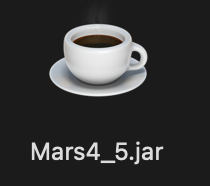
\includegraphics[width=0.15\textwidth]{1.png} 
        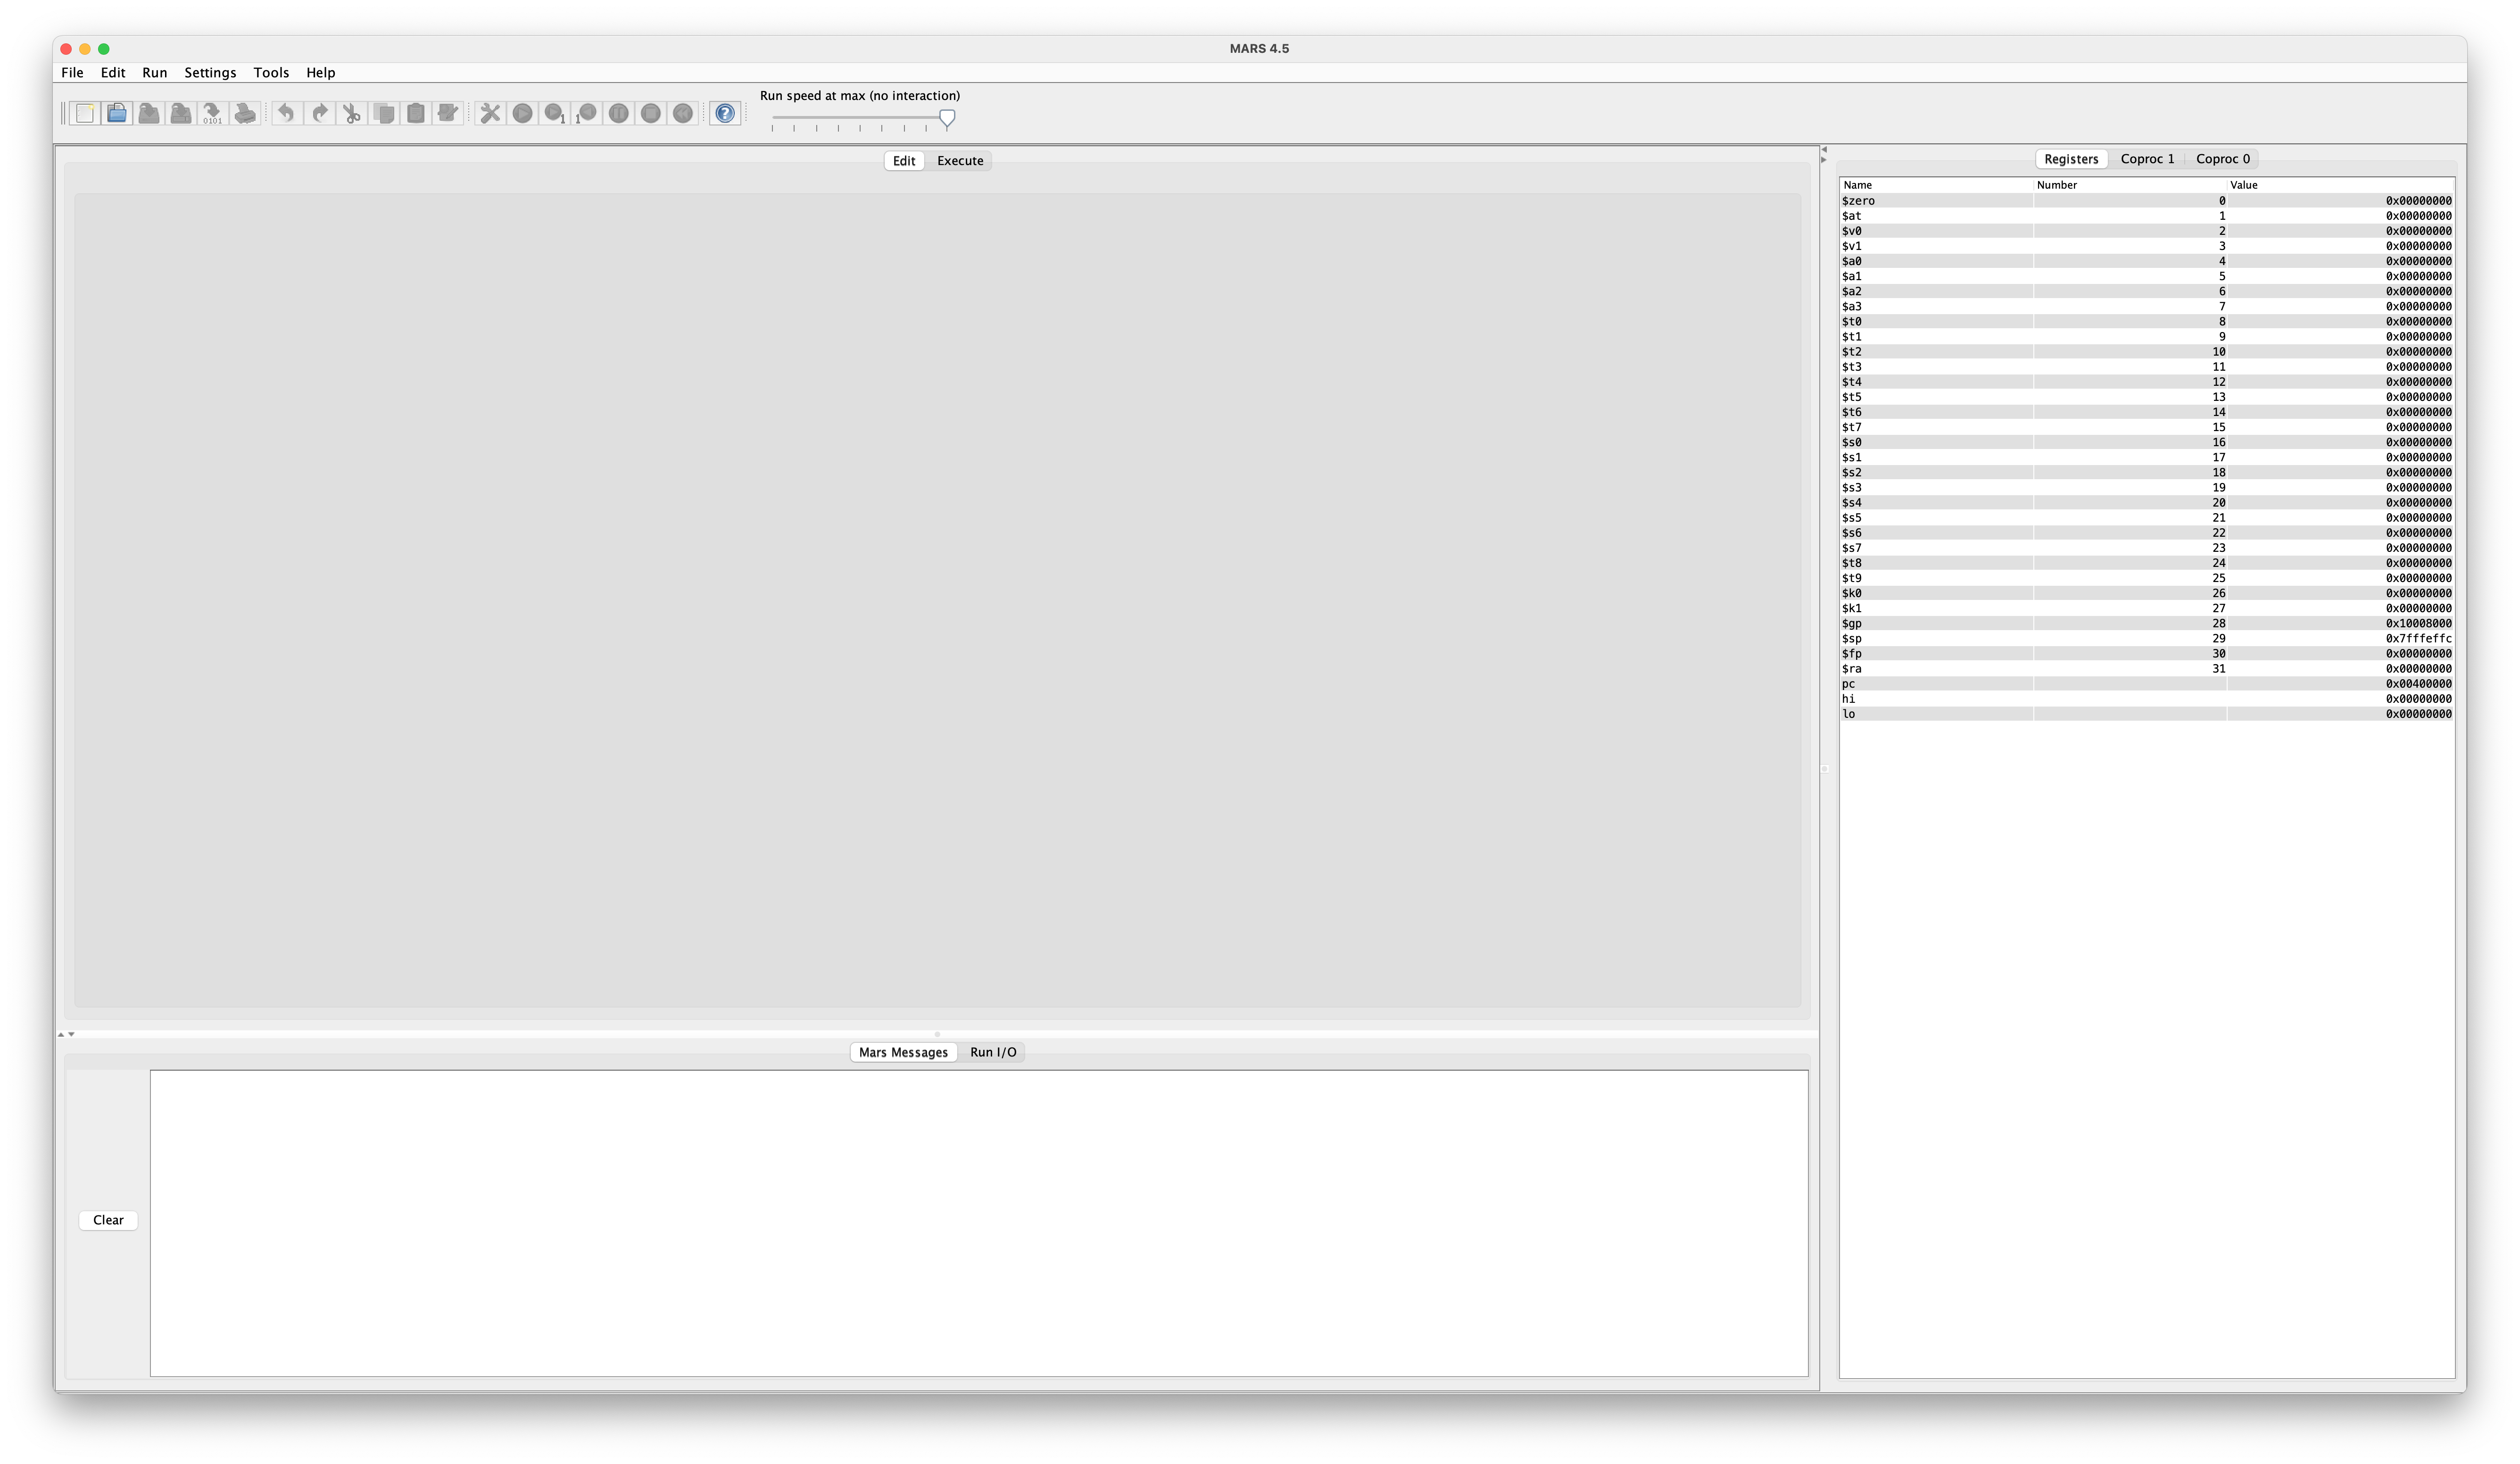
\includegraphics[width=0.9\textwidth]{2.png} 
    \end{center}
    
    \newpage
    \item Use the menubar File...Open or the Open icon 
\includegraphics[width=0.04\textwidth]{3.png} to open Fibonacci.asm in the default folder. (All icons have menubar equivalents; the remainder of these steps will use the icon whenever possible.)
    \begin{center}
        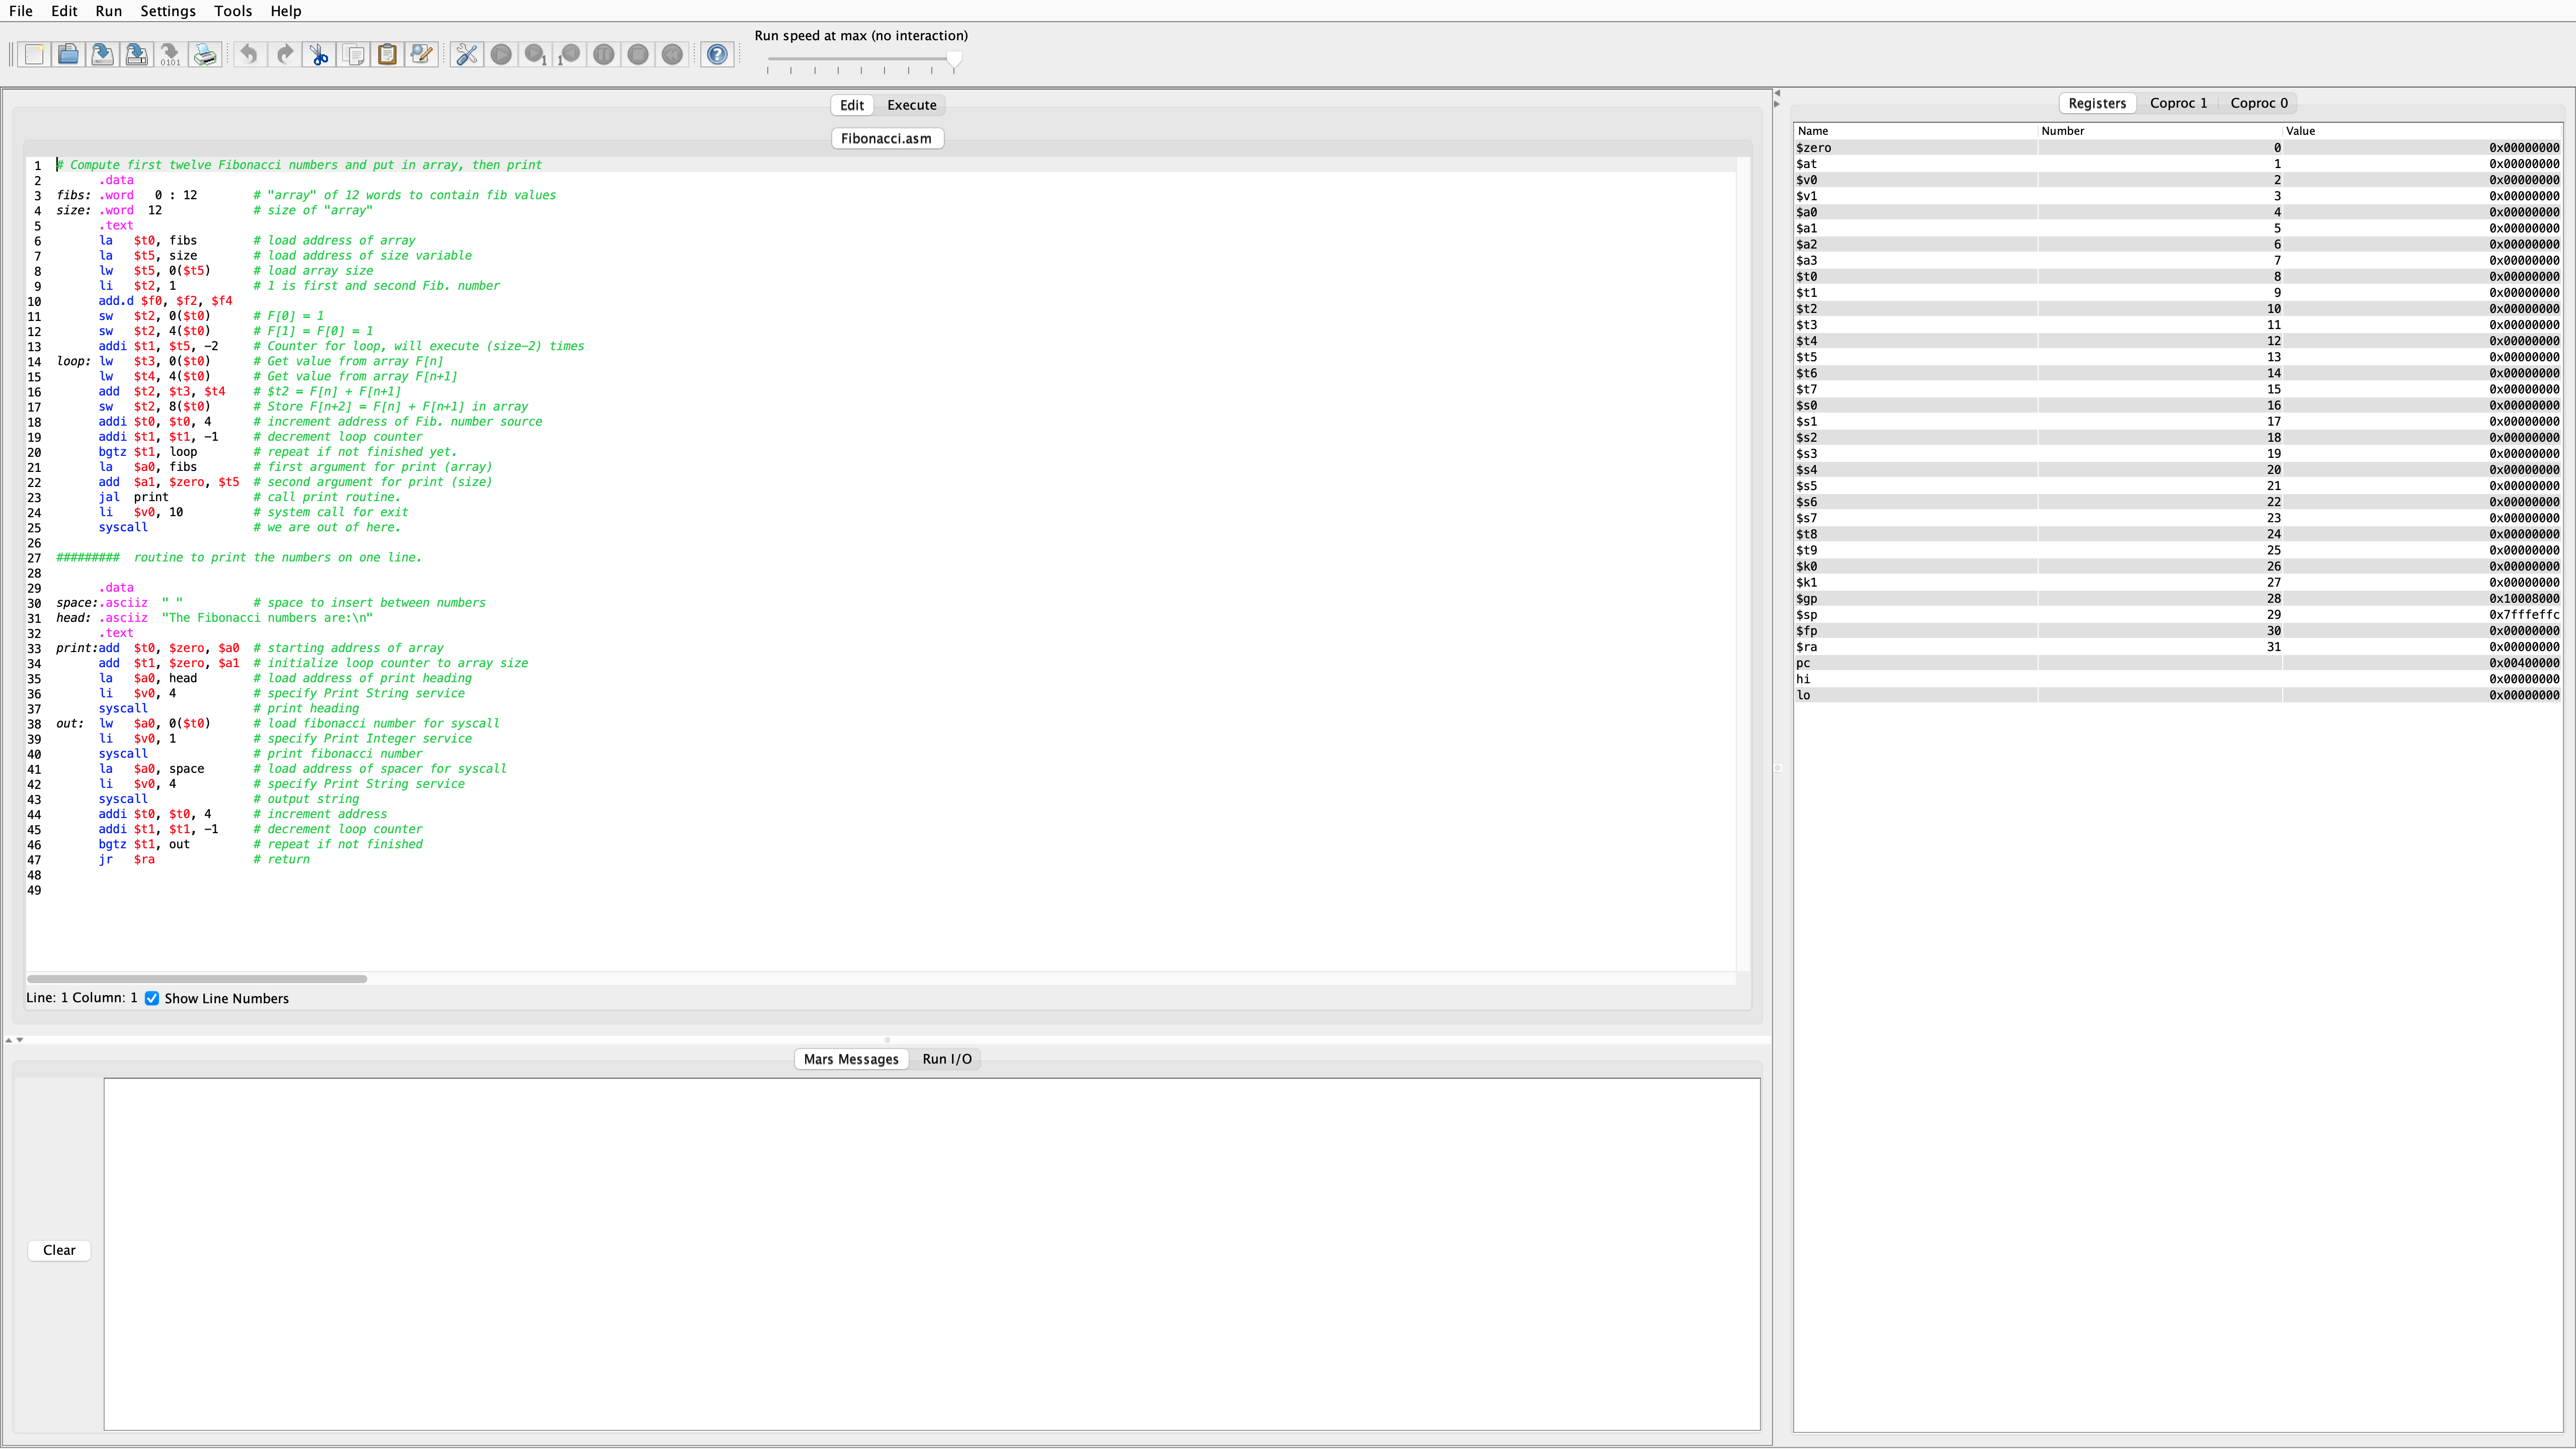
\includegraphics[width=0.9\textwidth]{4.png} 
    \end{center}
    
  \newpage
    \item The provided assembly program is complete. Assemble the program using the icon 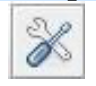
\includegraphics[width=0.04\textwidth]{5.png} 
    \begin{center}
        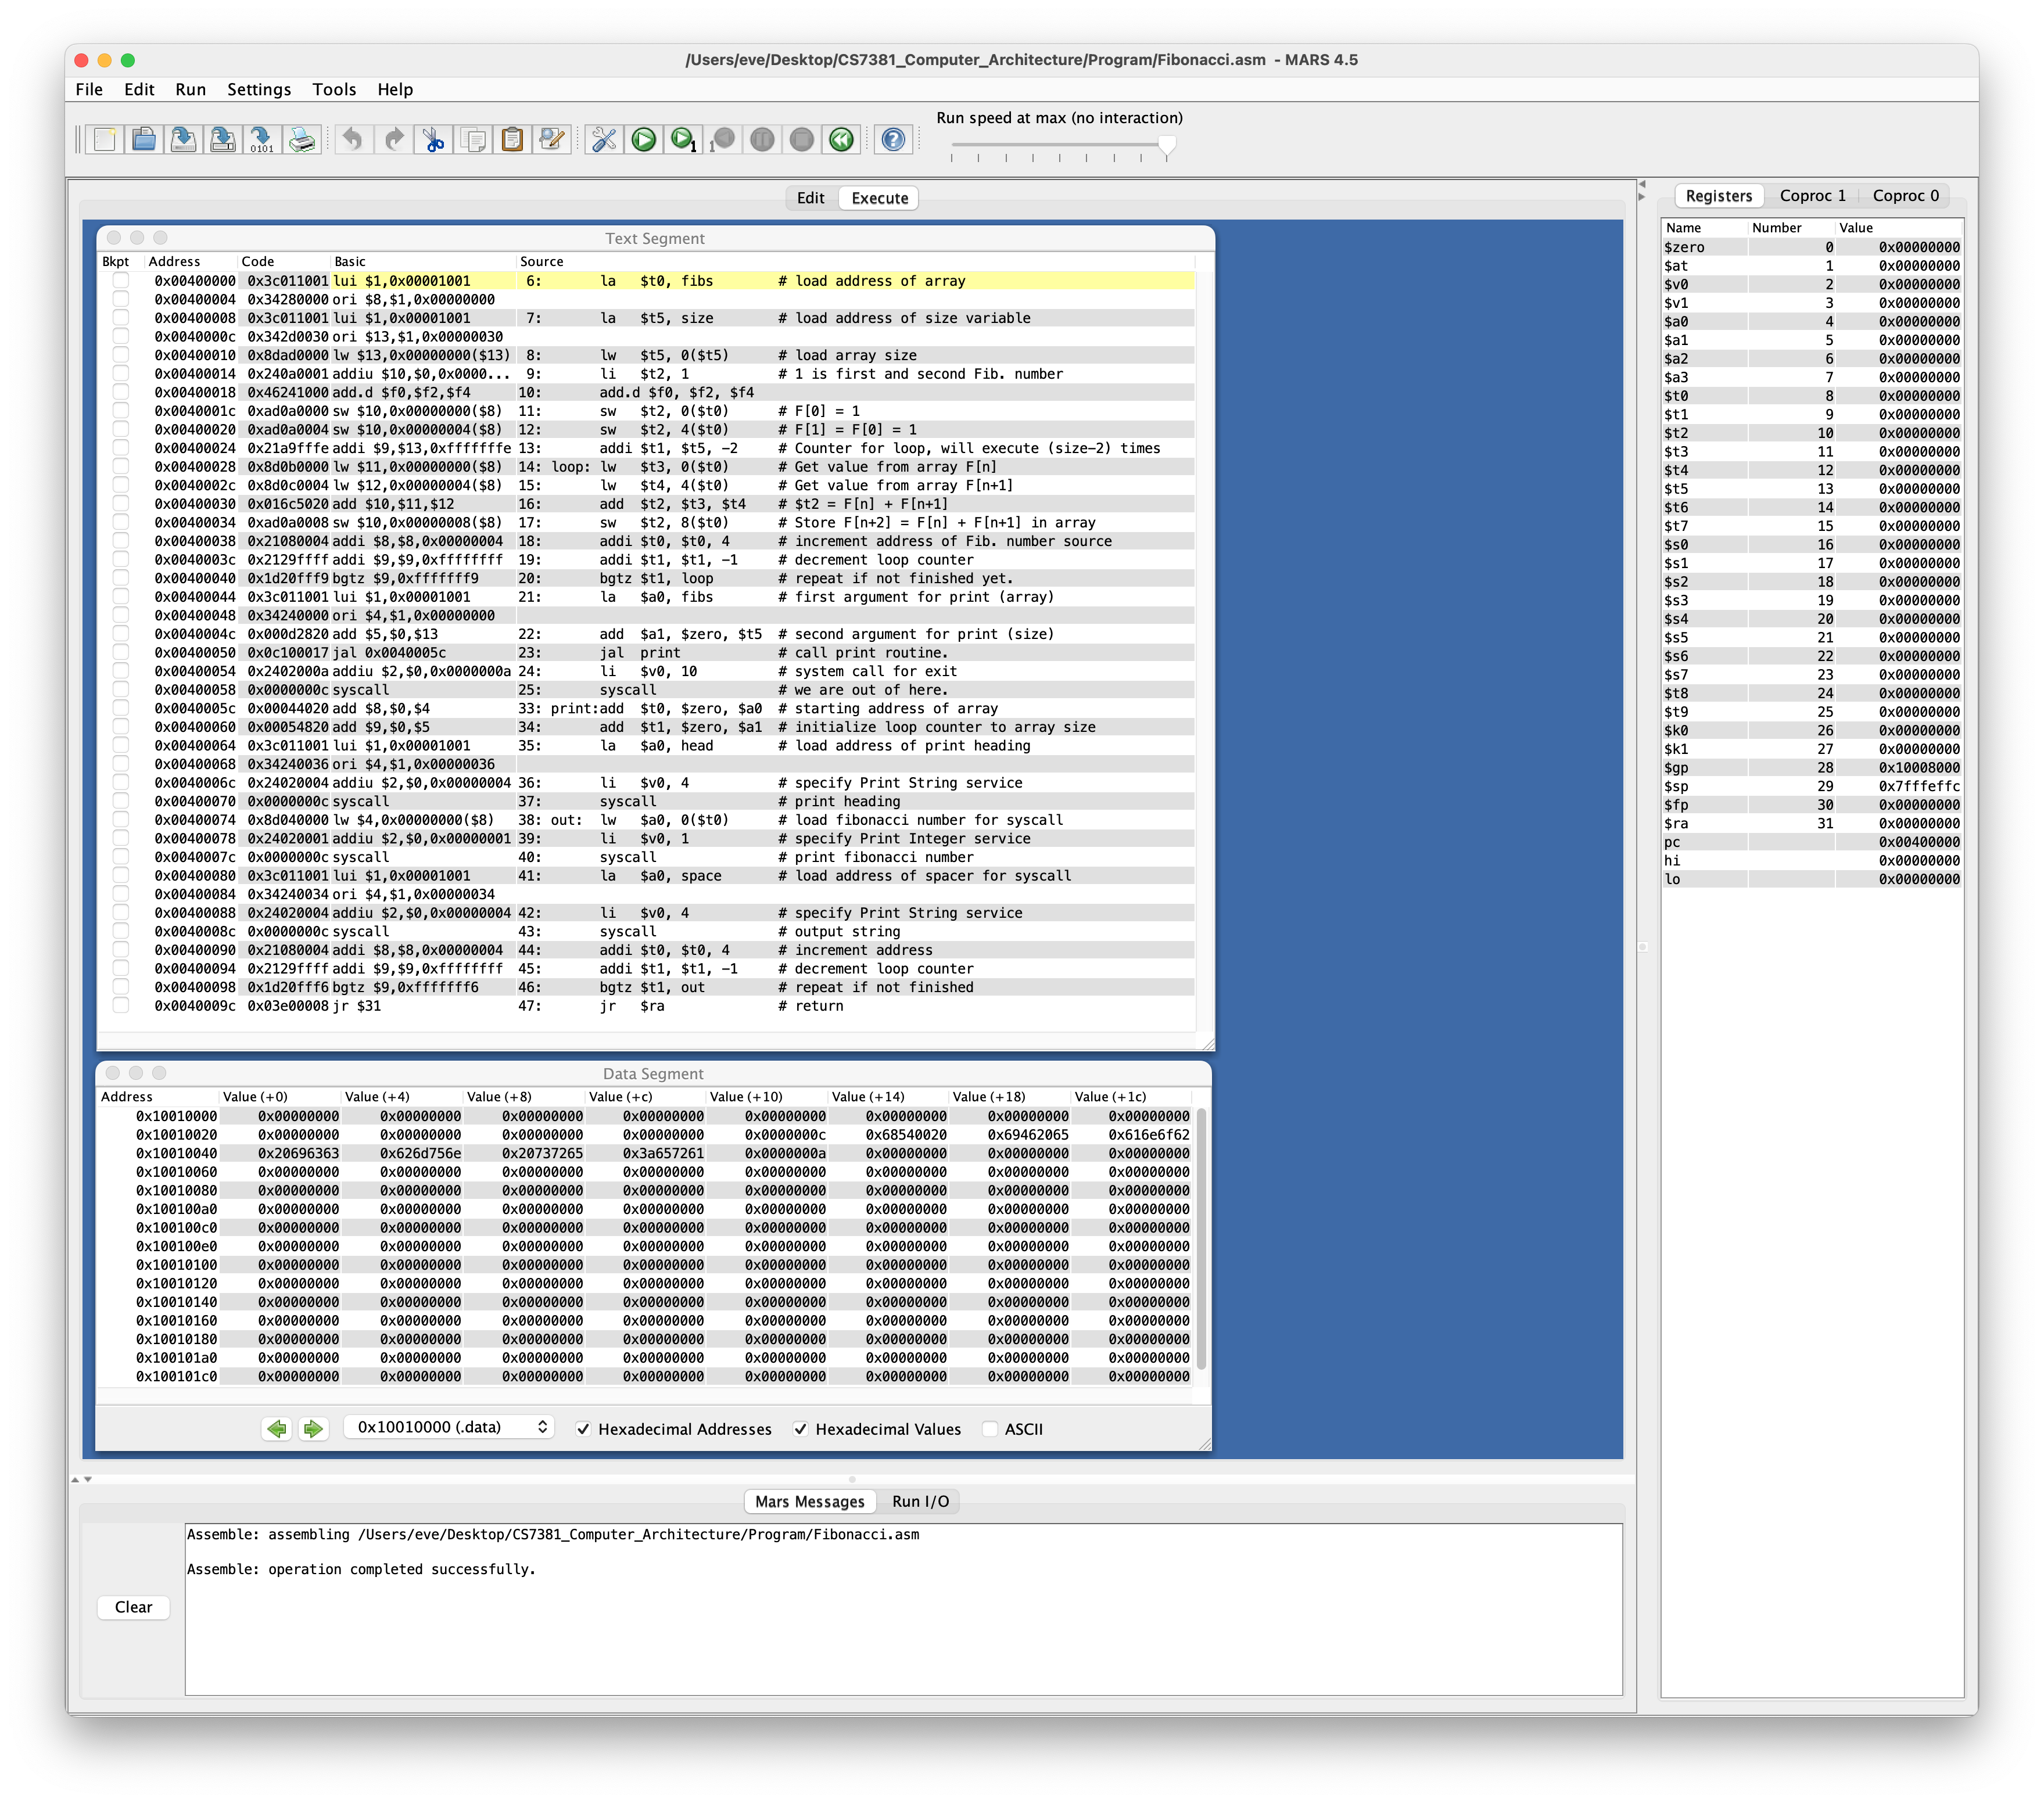
\includegraphics[width=0.9\textwidth]{6.png} 
    \end{center}

   \newpage
    \item Identify the location and values of the program’s initialized data. Use the checkbox to toggle the display format between decimal and hexadecimal 
\includegraphics[width=0.2\textwidth]{7.png}
    \begin{center}
        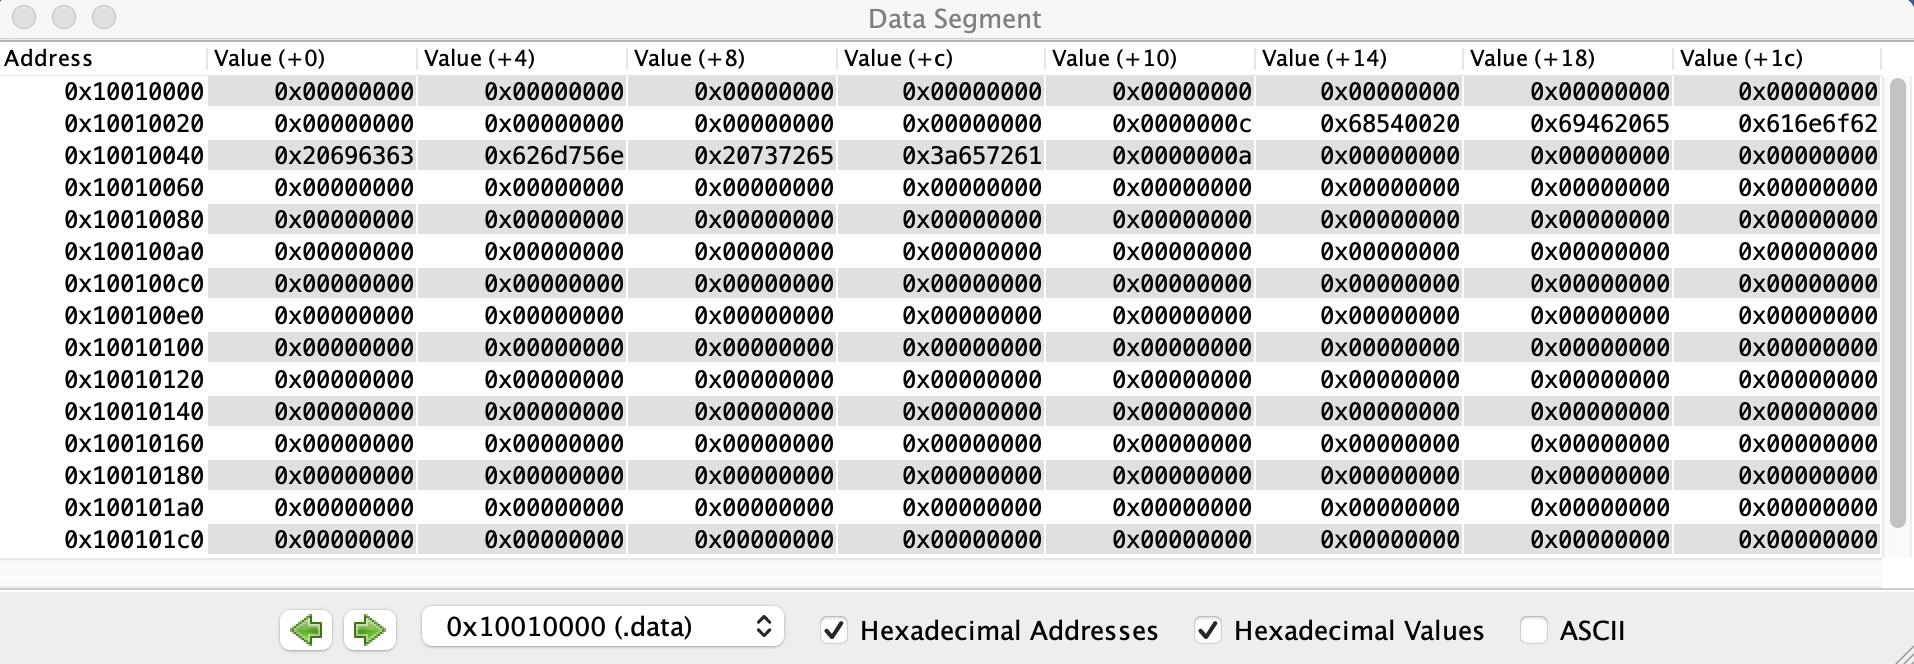
\includegraphics[width=0.9\textwidth]{8.png} 
        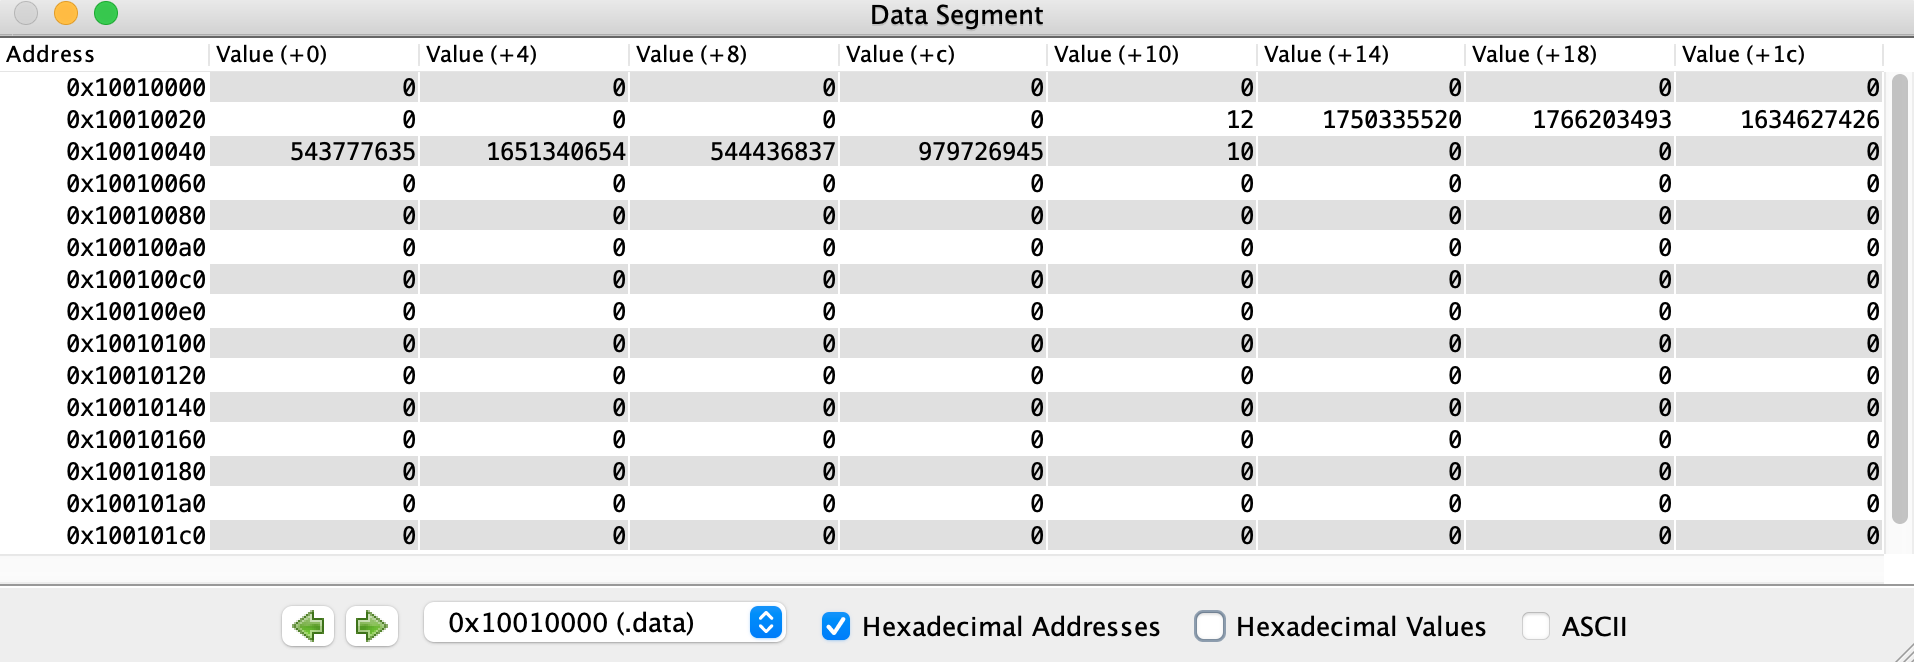
\includegraphics[width=0.9\textwidth]{9.png}
    \end{center}
    \begin{itemize}
        \item[$\bullet$] The twelve-element array fibs is initialized to zero, at addresses 0x10010000 ...0x1001002c.
        \begin{center}
            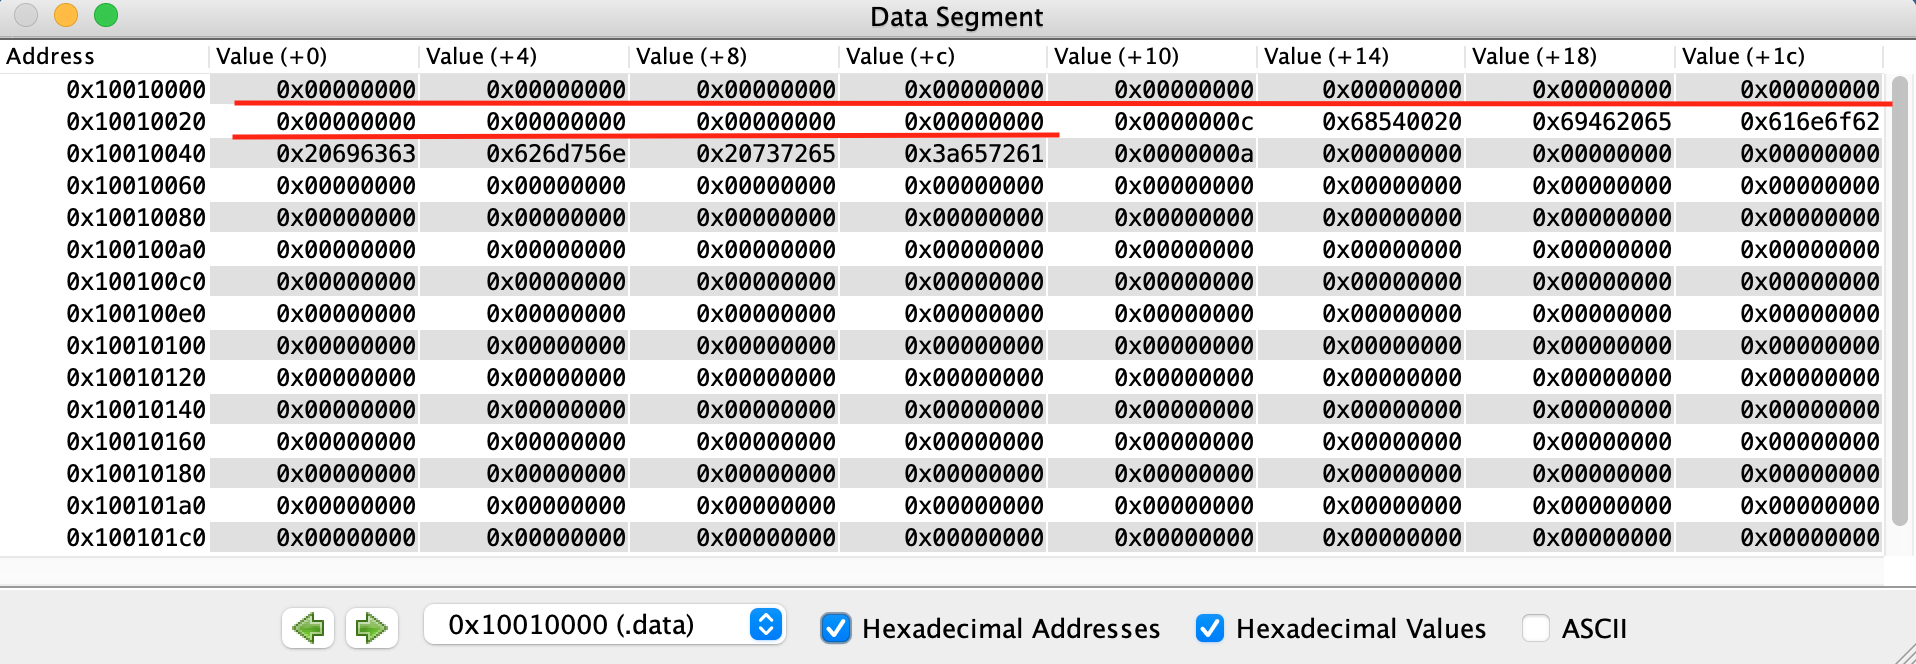
\includegraphics[width=0.85\textwidth]{10.png}
        \end{center}
        \item[$\bullet$] The data location size has value $12_{10} (C_{16})$ at 0x10010030.  Use the checkbox to toggle the display format between decimal and hexadecimal 
\includegraphics[width=0.2\textwidth]{7.png}.
        \begin{center}
            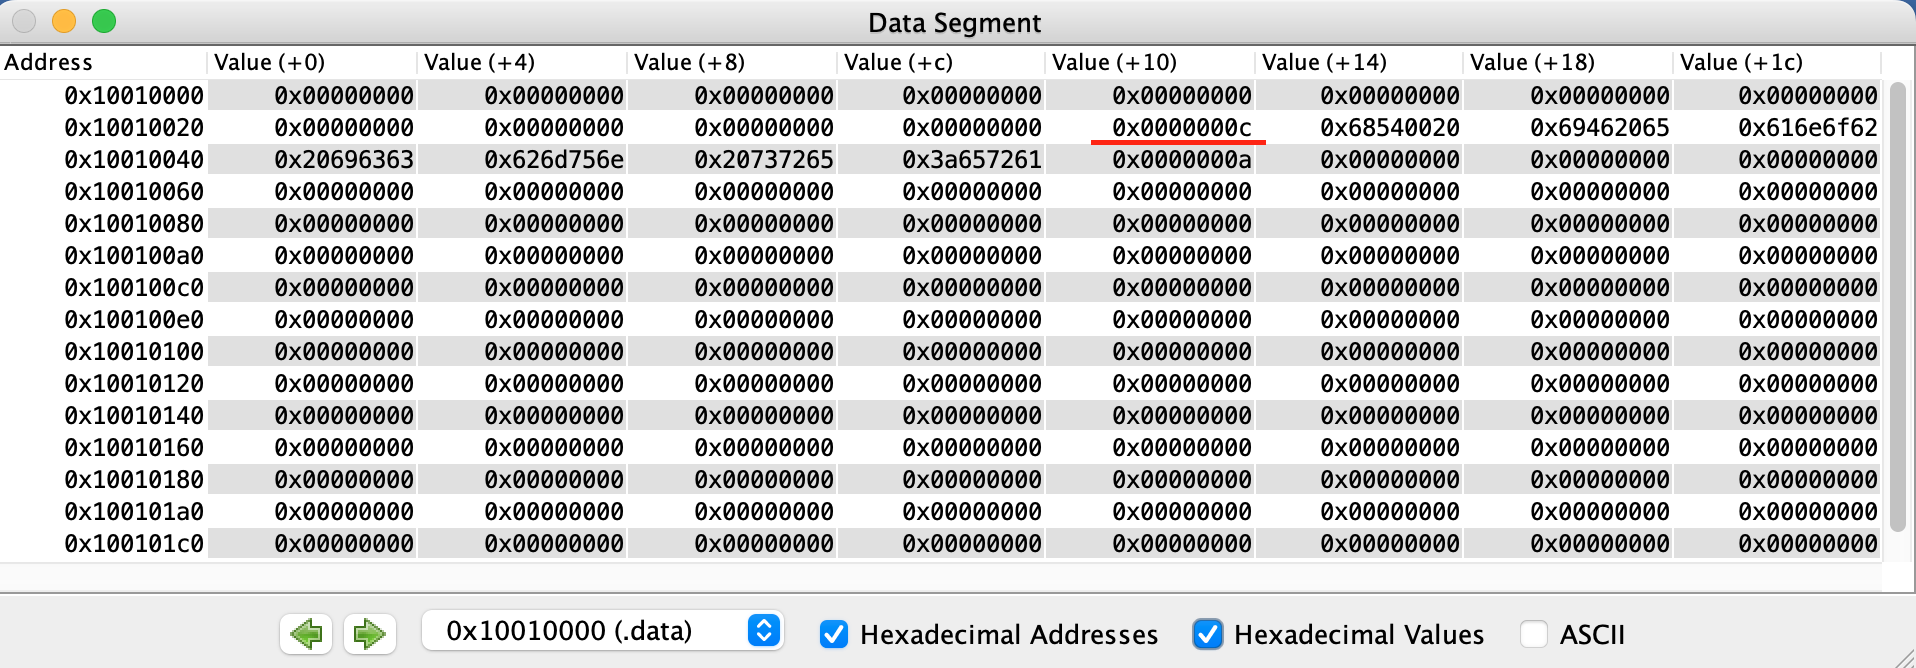
\includegraphics[width=0.85\textwidth]{12.png}
            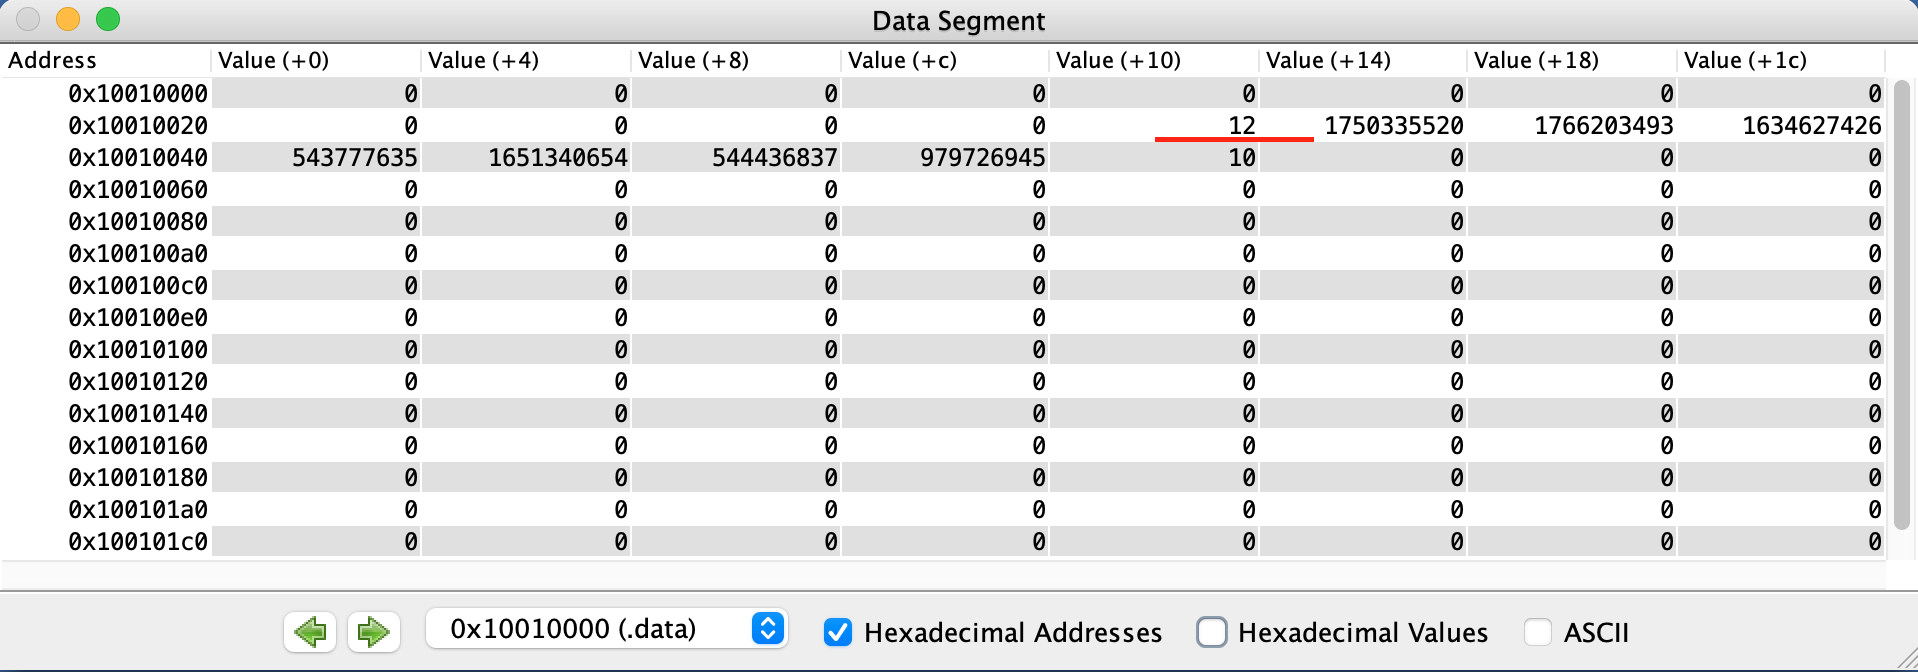
\includegraphics[width=0.85\textwidth]{13.png}
        \end{center}
    \end{itemize}

      \newpage
    \item Locate the Registers display, which shows the 32 common MIPS registers. Other tabs in the Registers display show the floating-point registers (Coproc 1) and status codes (Coproc 0).\\
    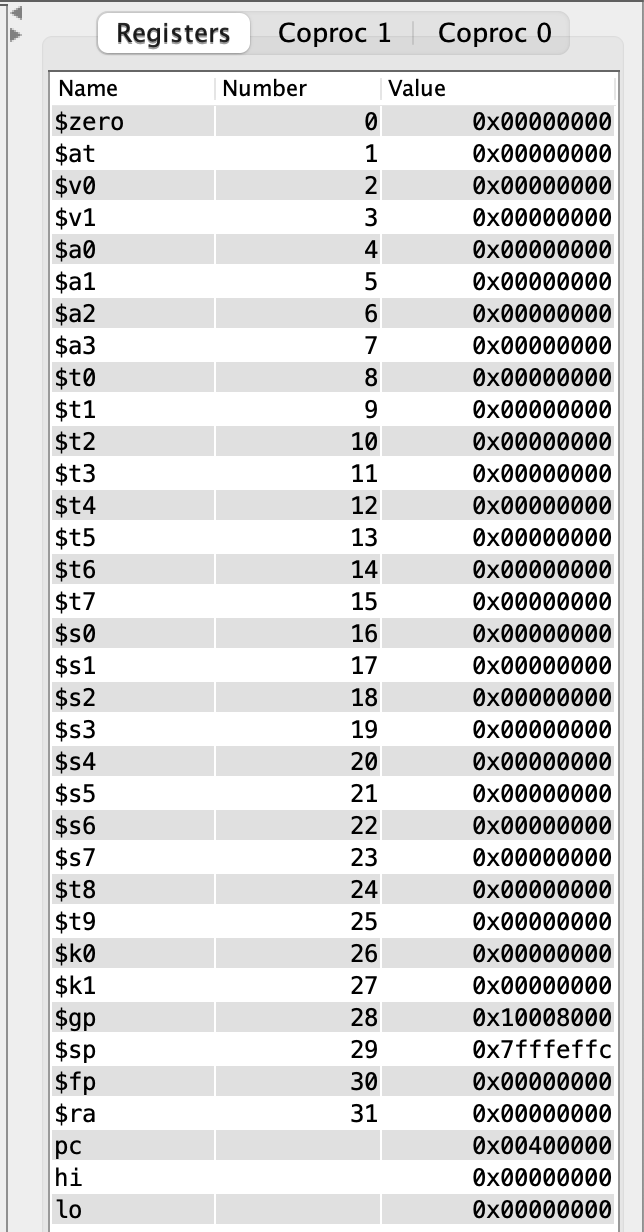
\includegraphics[width=0.25\textwidth]{14.png} \ \ \ \
    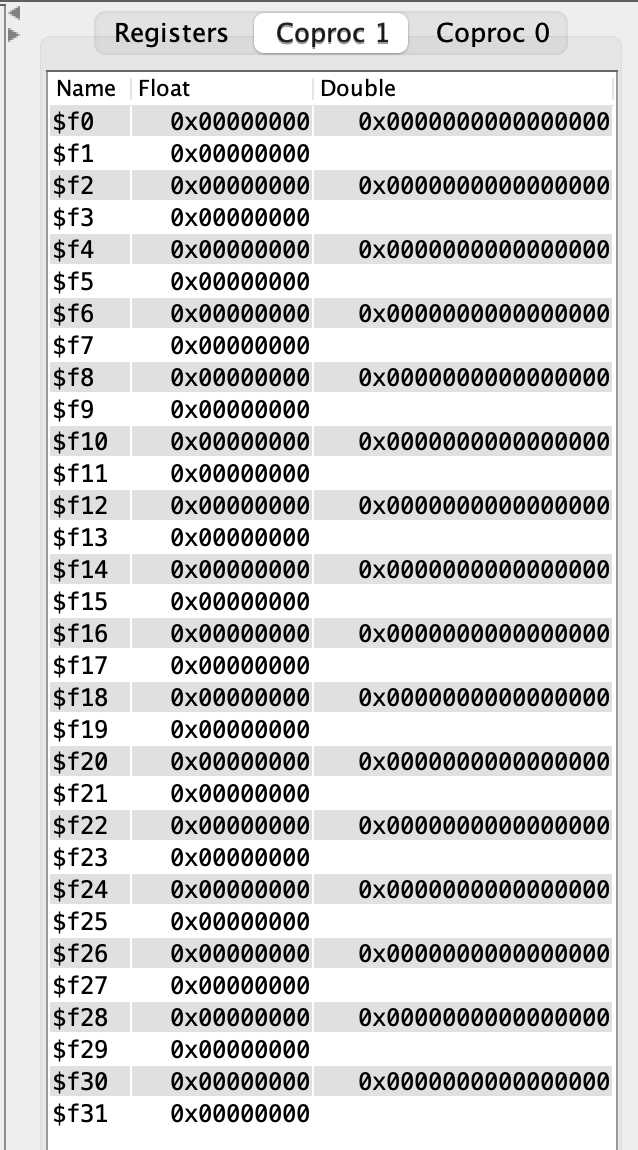
\includegraphics[width=0.25\textwidth]{15.png} \ \ \ \
    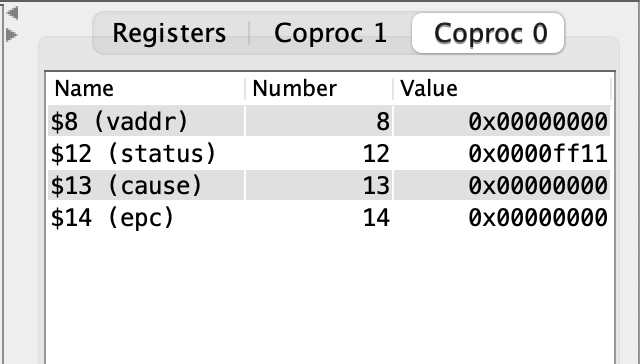
\includegraphics[width=0.25\textwidth]{16.png}
   
 
    \item Use the slider bar to change the run speed to about 10 instructions per second. This allows us to “watch the action” instead of the assembly program finishing directly.
    \begin{center}
            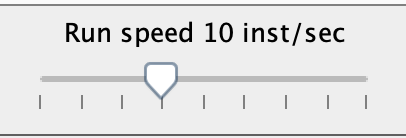
\includegraphics[width=0.2\textwidth]{17.png}
    \end{center}
    
     \newpage
    \item Choose how you will execute the program:\\
    The icon 
\includegraphics[width=0.04\textwidth]{18.png} runs the program to completion. Using this icon, you should observe the yellow highlight showing the program’s progress and the values of the Fibonacci sequence appearing in the Data Segment display.
    \begin{center}
            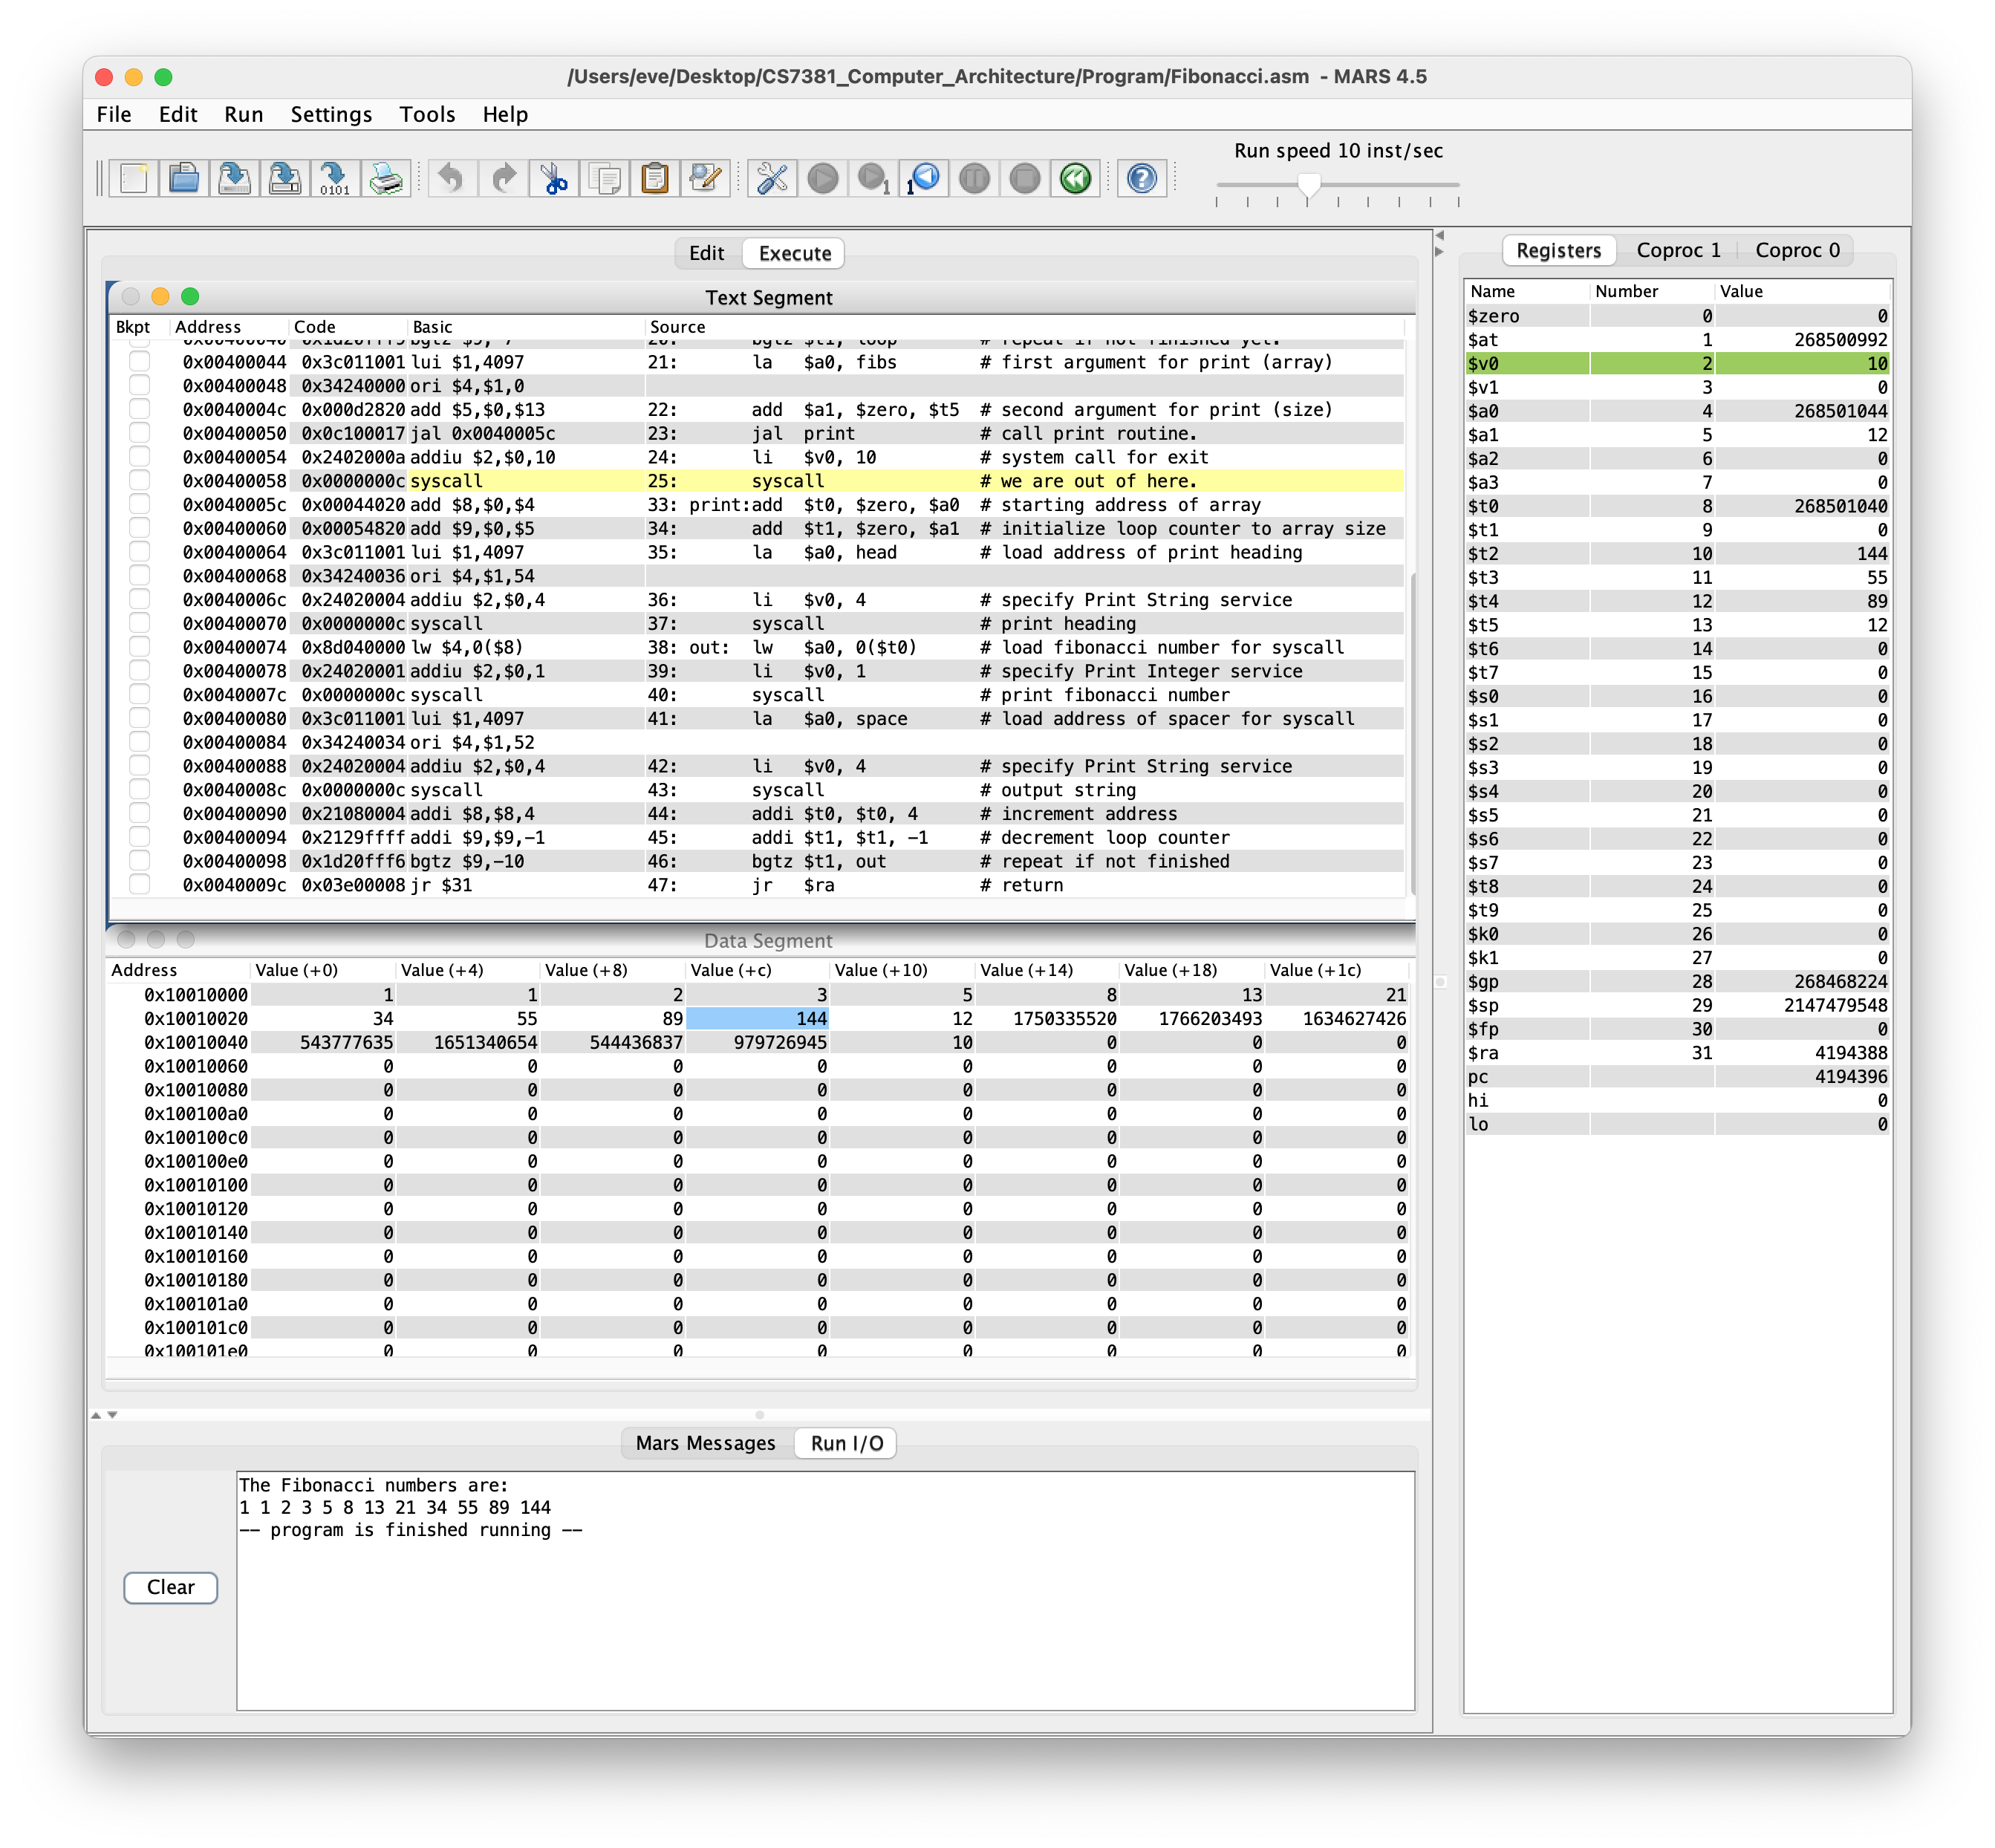
\includegraphics[width=0.9\textwidth]{19.png}
    \end{center}

    \begin{itemize}
        \newpage
        \item[$\bullet$] The 
\includegraphics[width=0.04\textwidth]{20.png} icon resets the program and simulator to initial values. Memory contents are those specified within the program, and register contents are generally zero. 
        \begin{center}
            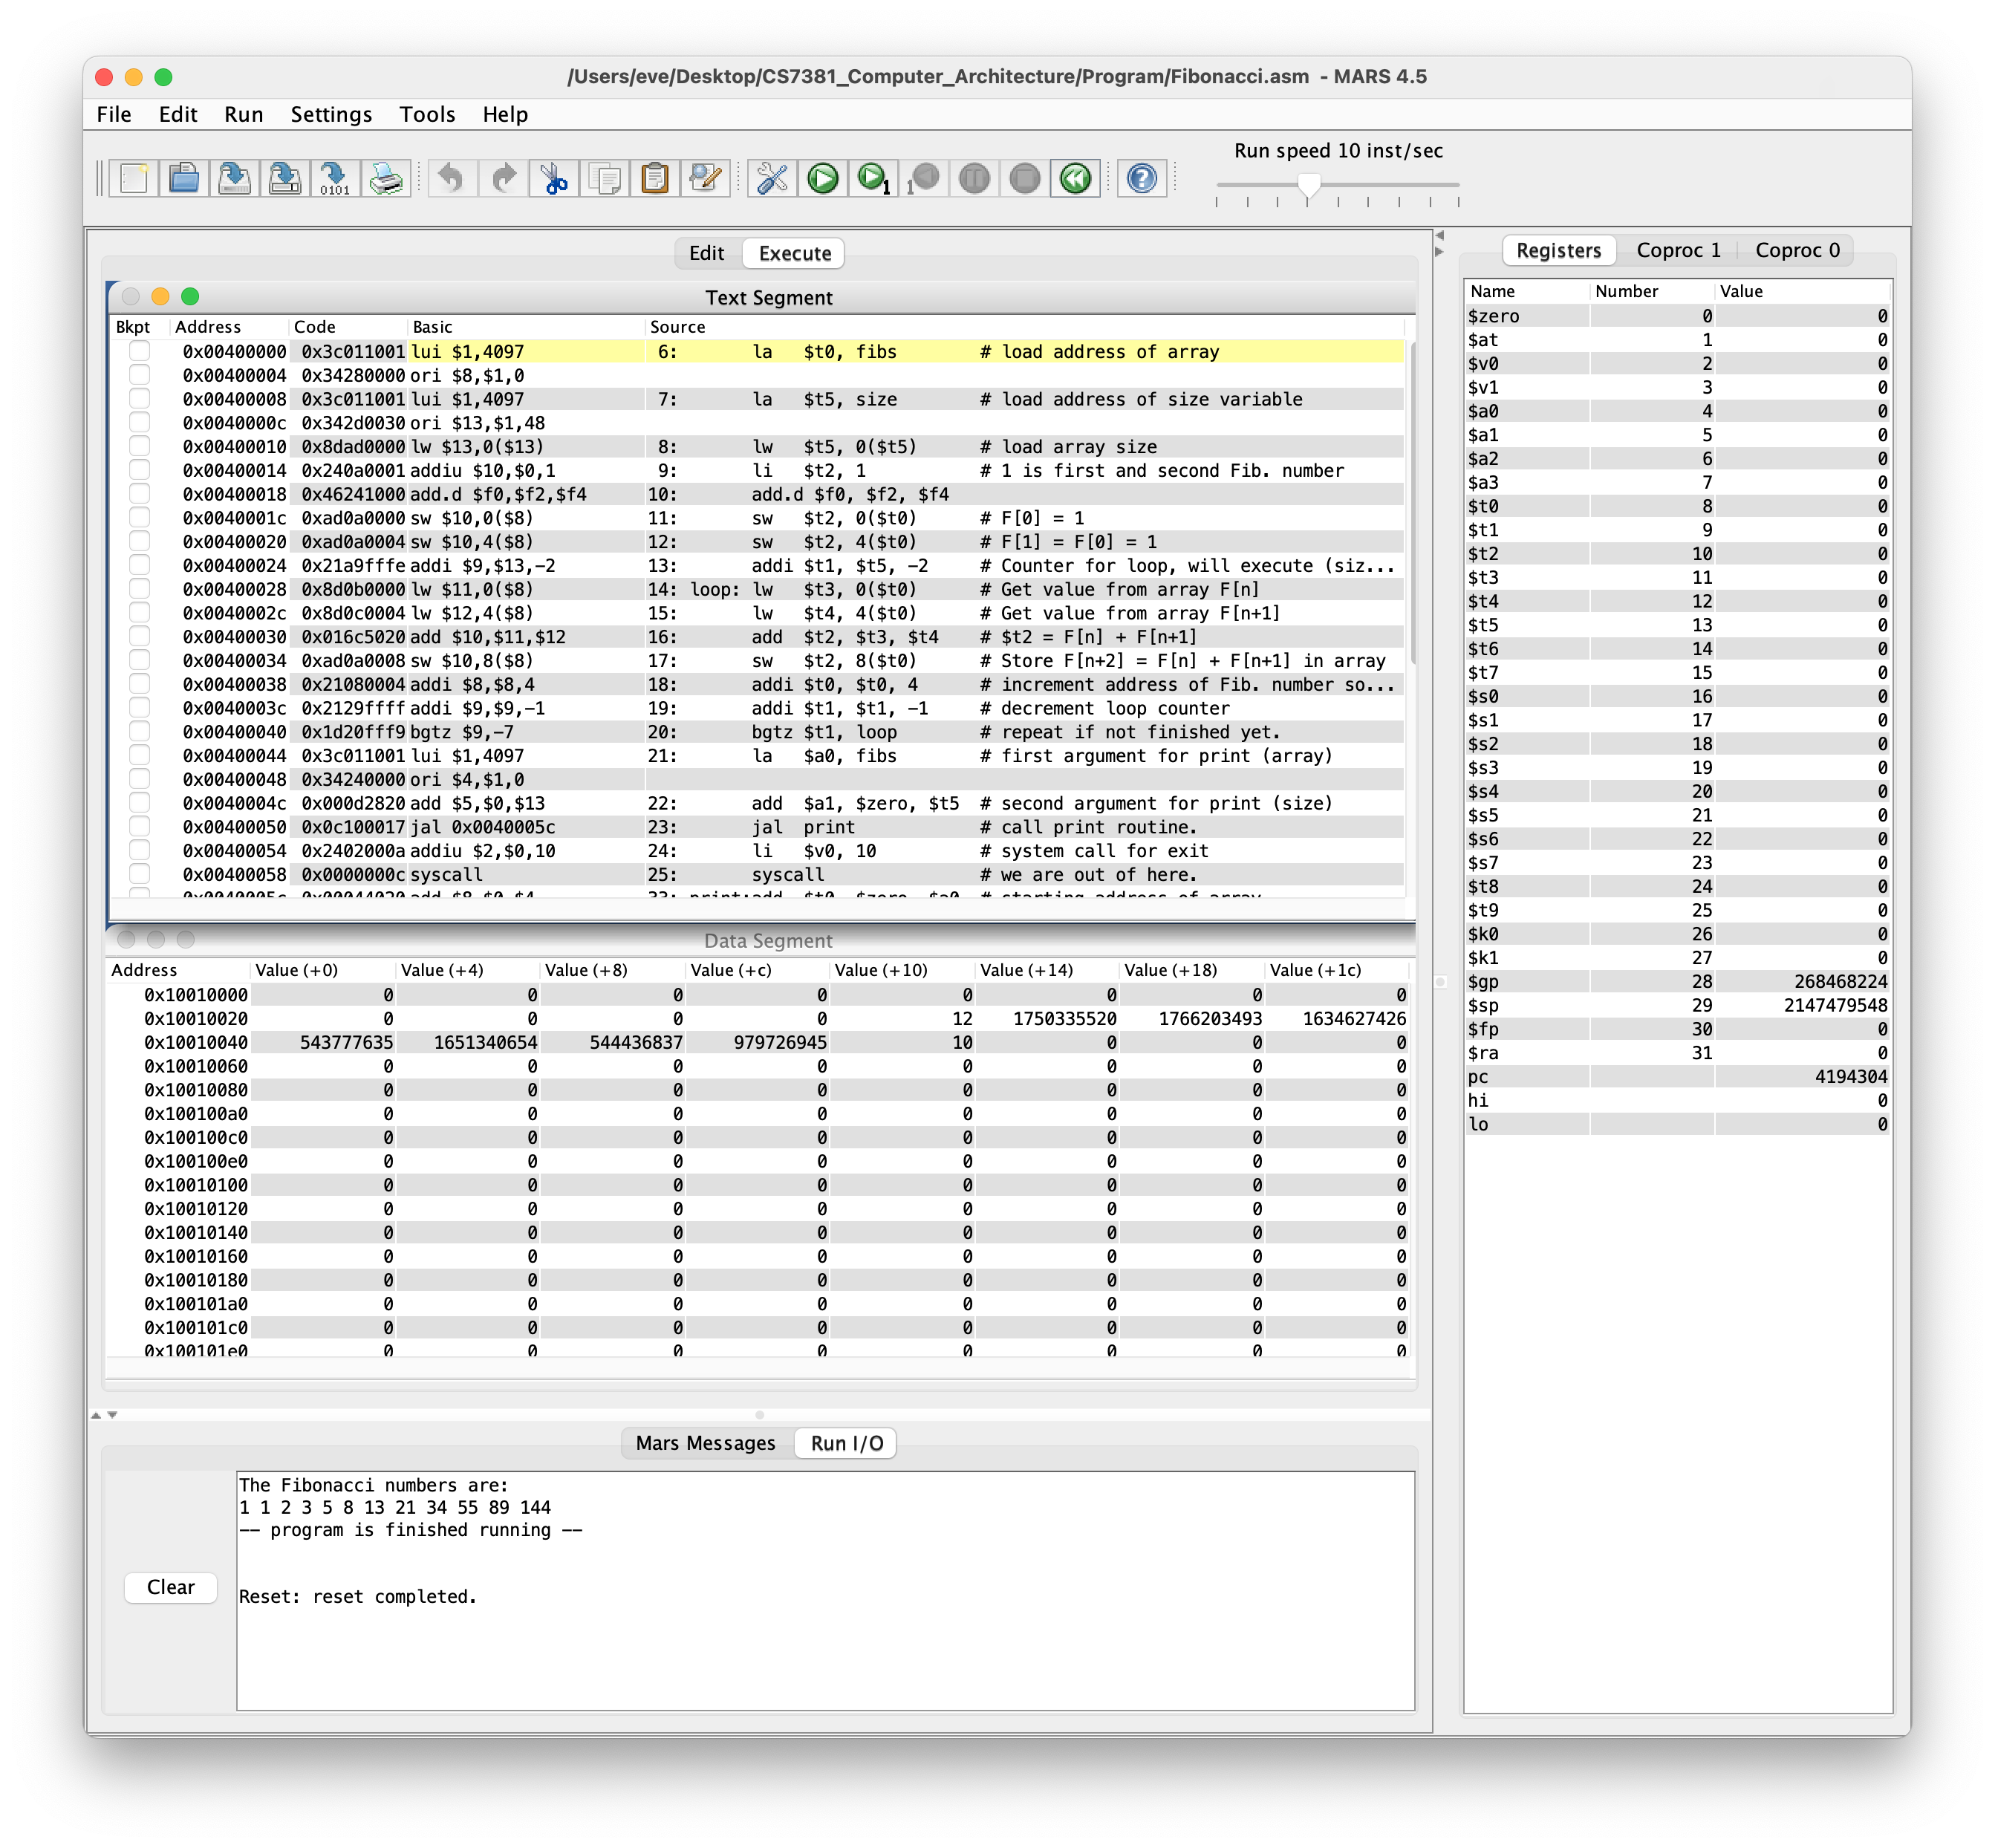
\includegraphics[width=0.9\textwidth]{21.png}
         \end{center}

        \newpage
         \item[$\bullet$] The 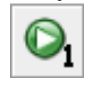
\includegraphics[width=0.04\textwidth]{22.png} icon is “single-step.” Its complement is 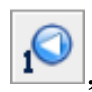
\includegraphics[width=0.04\textwidth]{23.png}, “single-step backwards” (undoes each operation).
        \begin{center}
            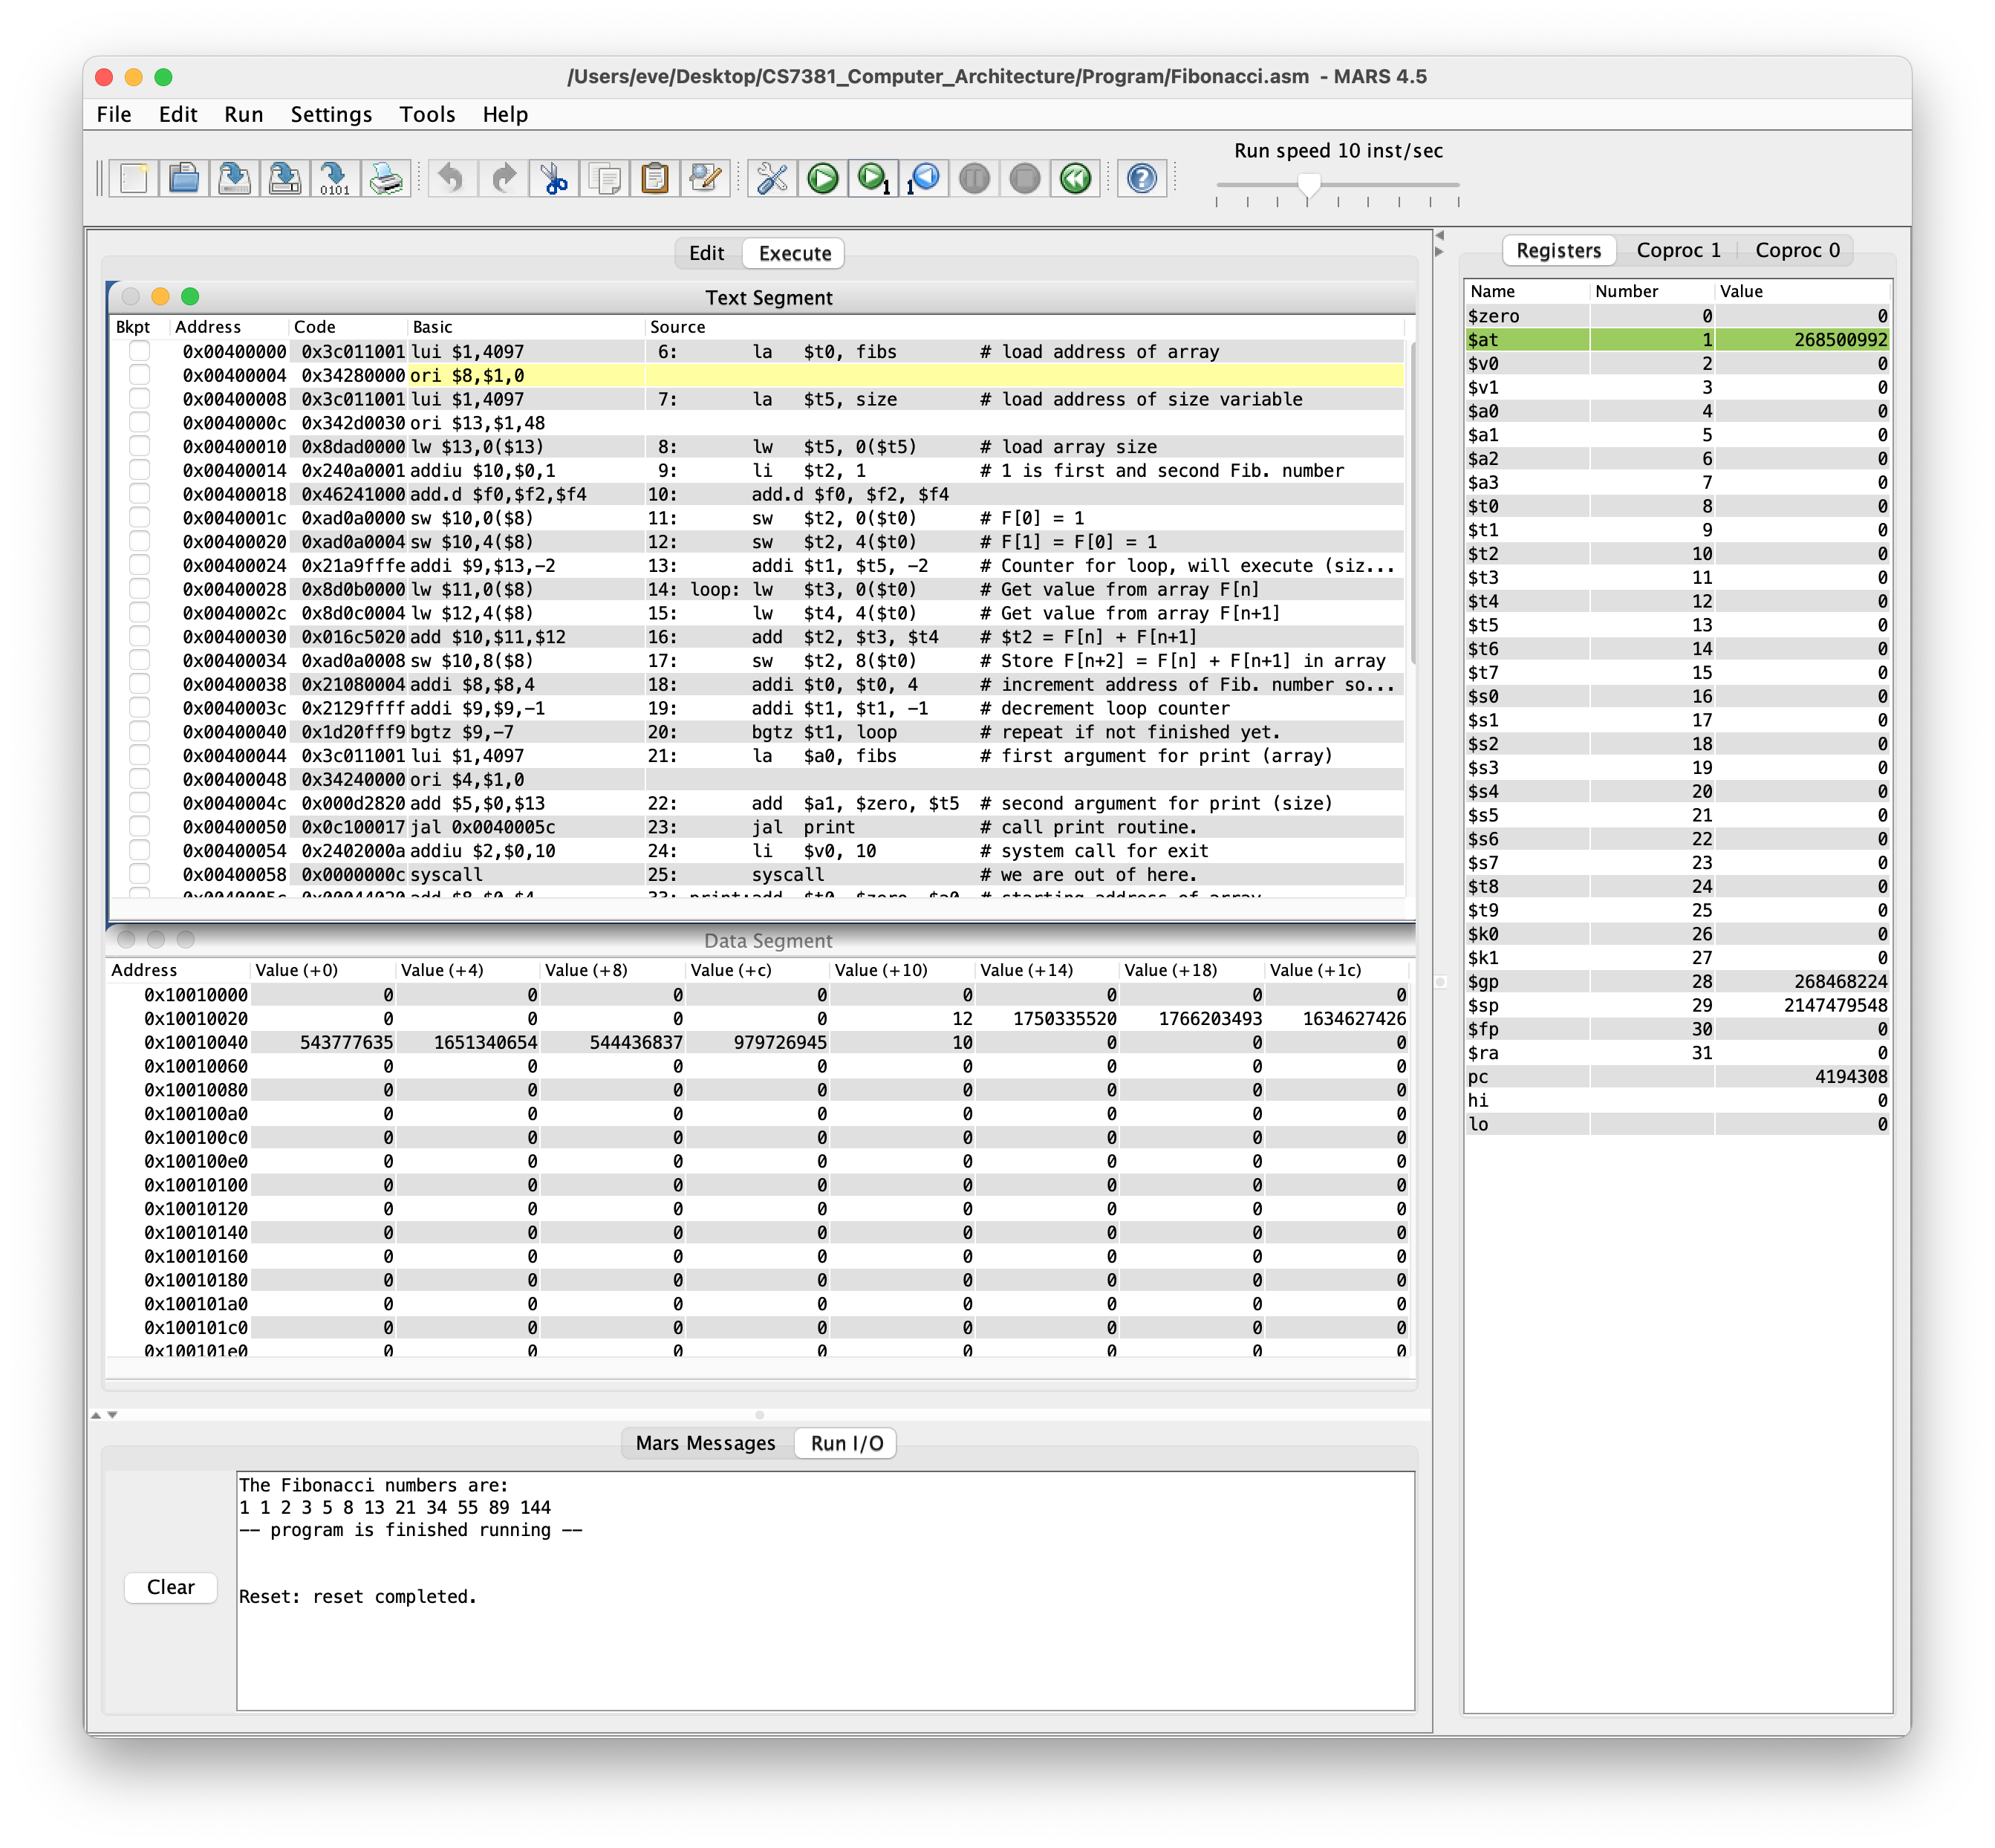
\includegraphics[width=0.9\textwidth]{24.png}
            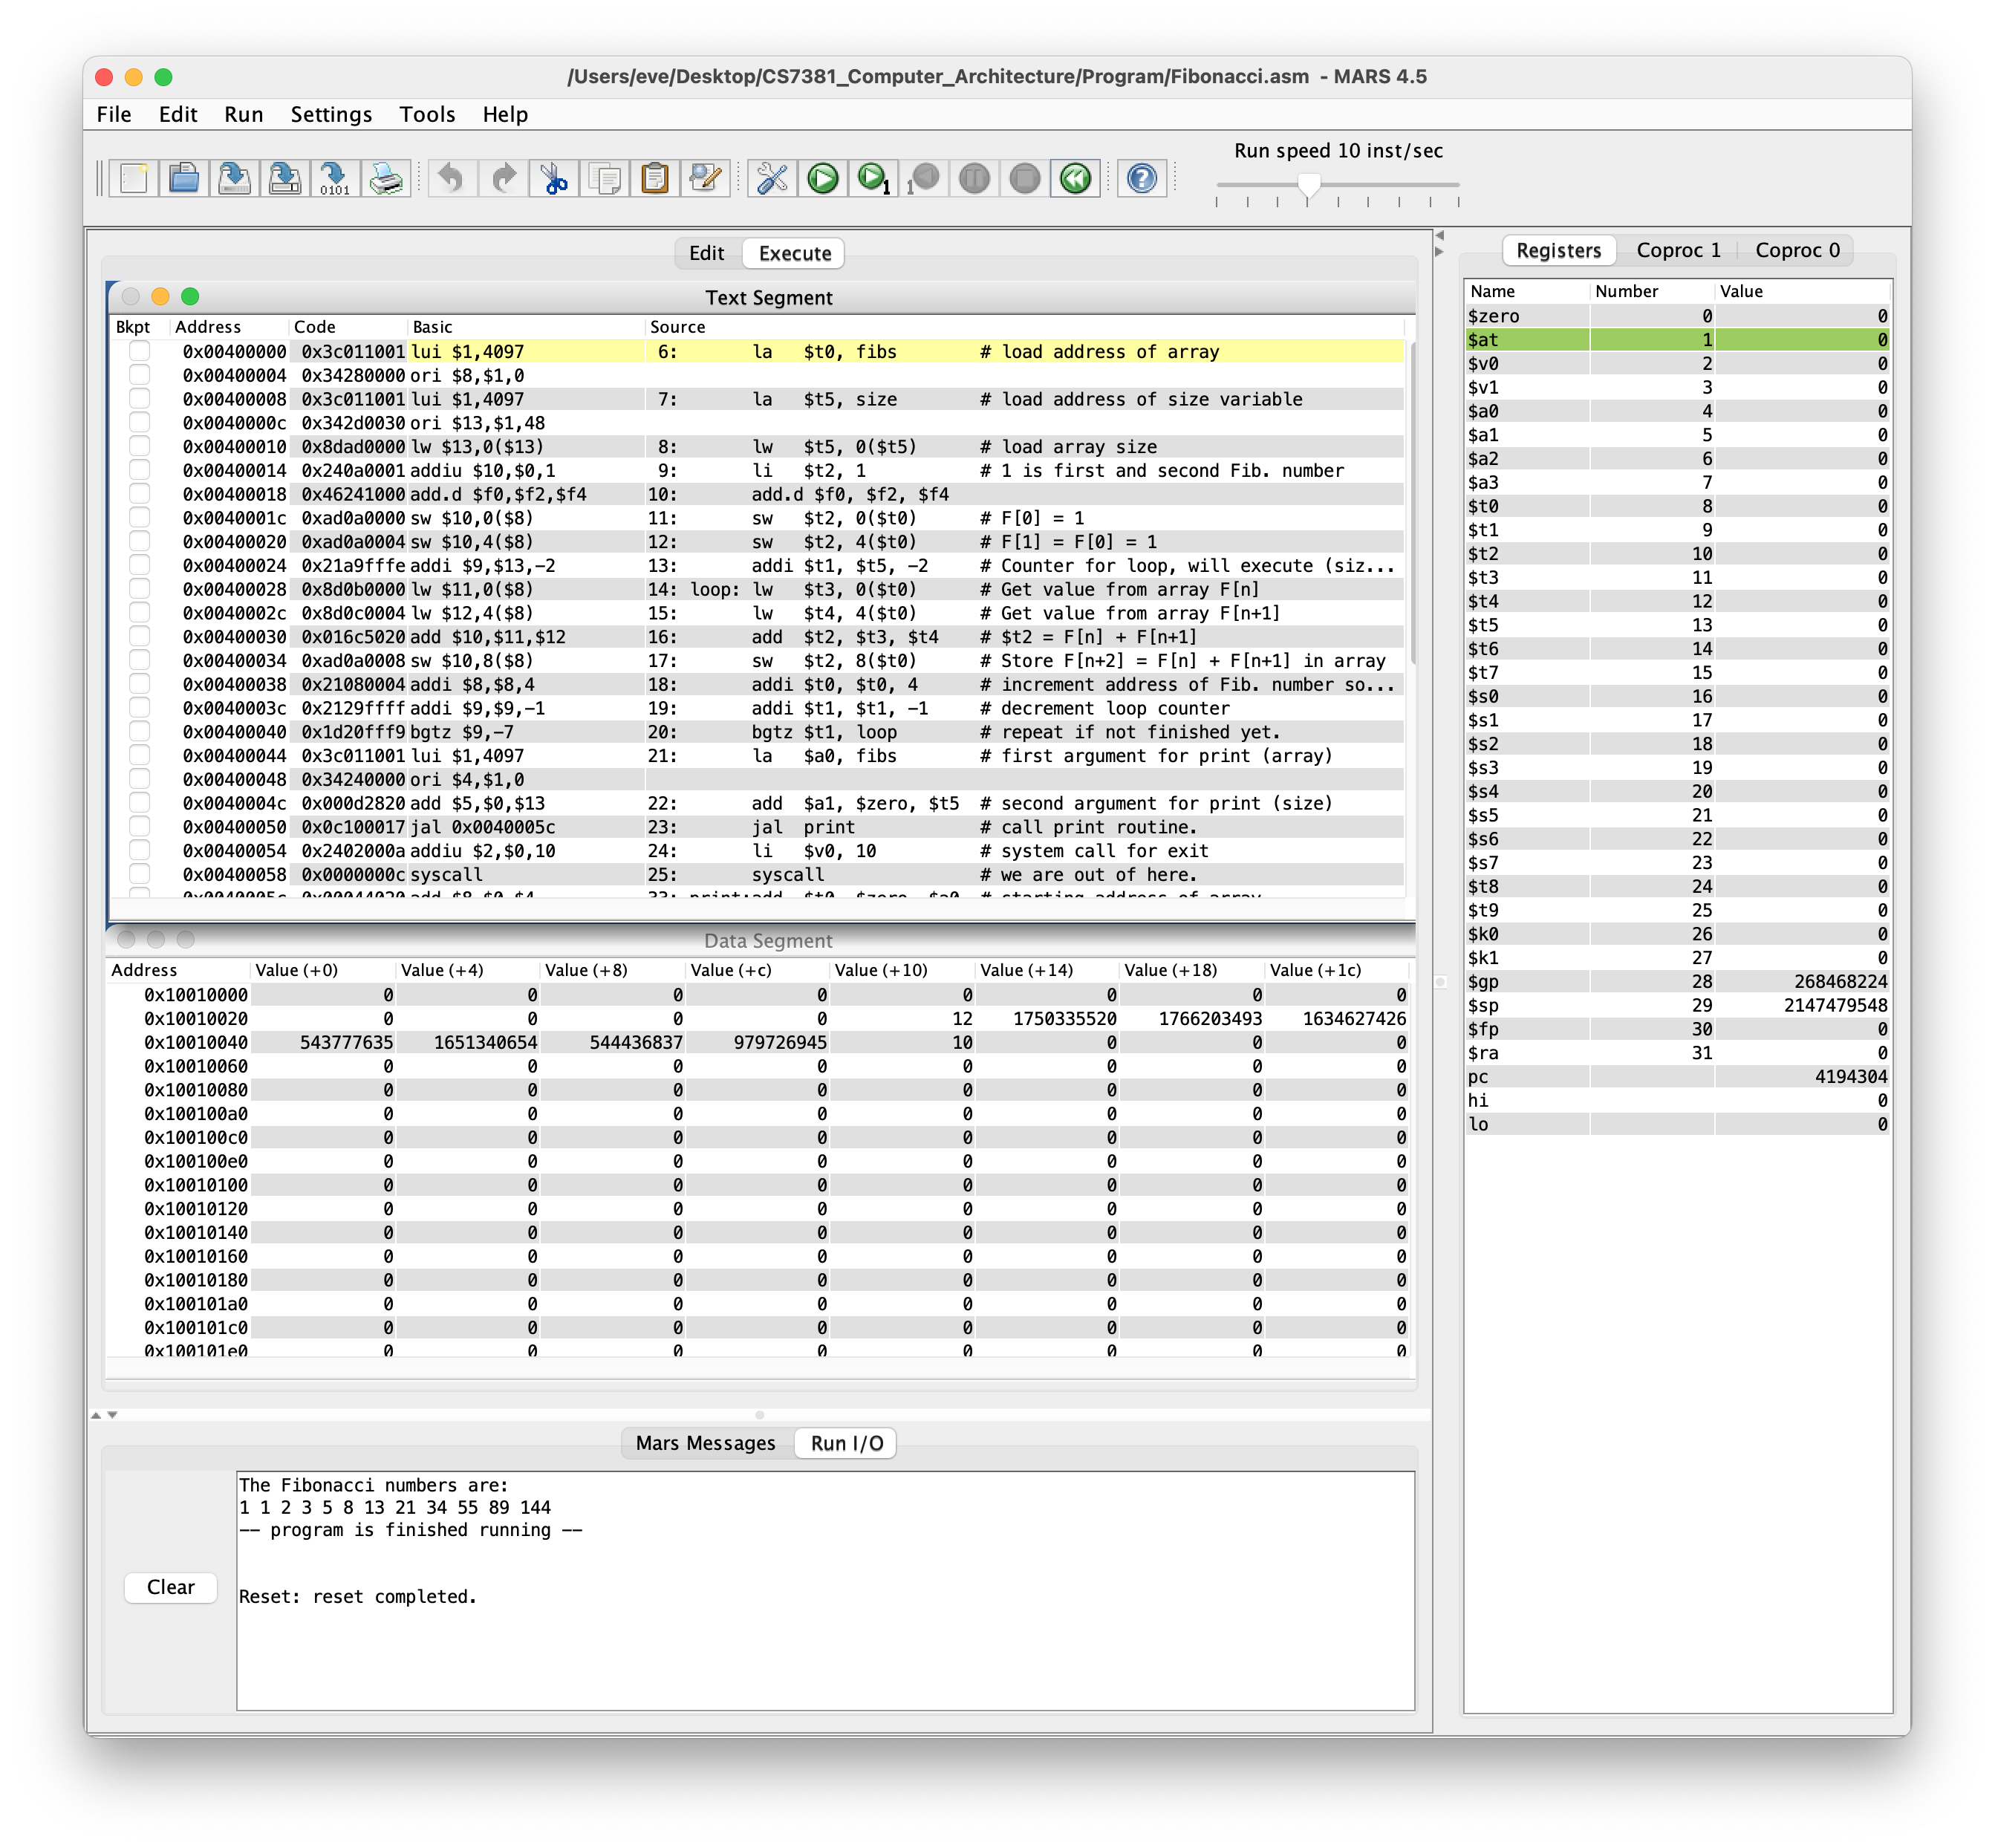
\includegraphics[width=0.9\textwidth]{25.png}
         \end{center}

        
    \end{itemize}
    \newpage
    \item Observe the output of the program in the Run I/O display window:\\
    The Fibonacci numbers are:\\
    1 1 2 3 5 8 13 21 34 55 89 144 \\
    -- program is finished running -- \\
            \begin{center}
            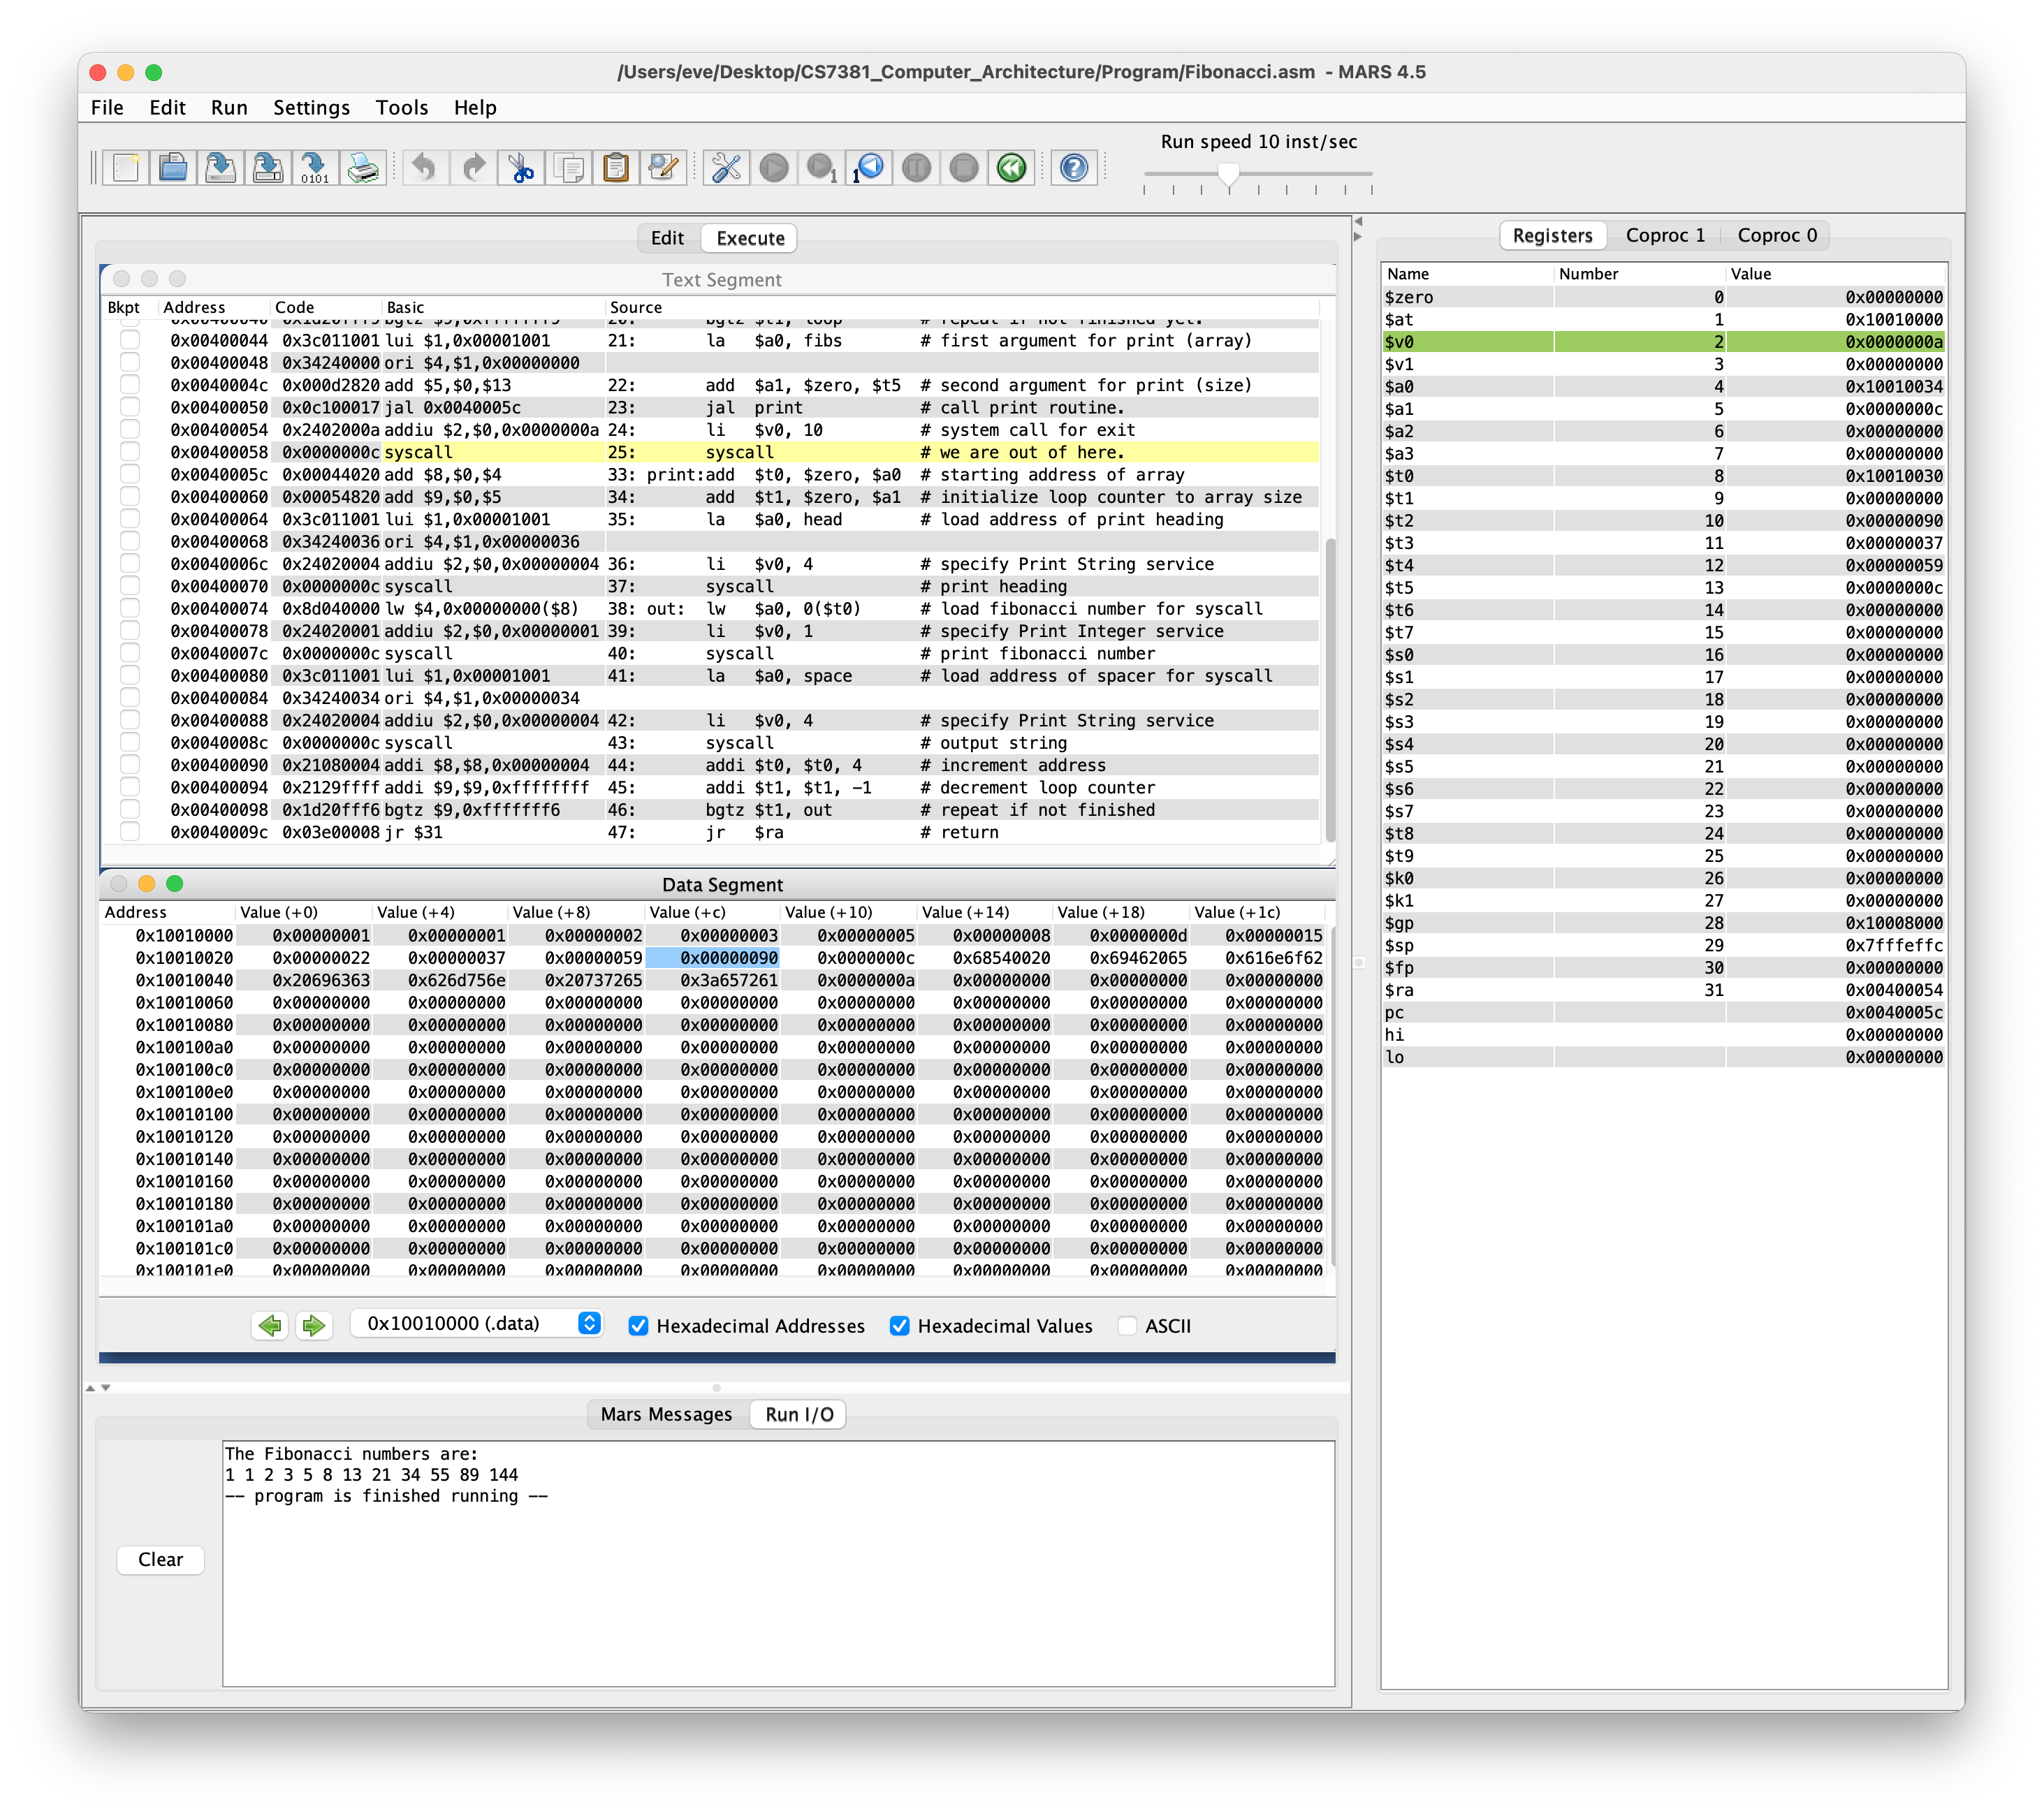
\includegraphics[width=0.9\textwidth]{26.png}
         \end{center}
    \newpage
    \item Modify the contents of memory. (Modifying a register value is exactly the same.)
    \begin{itemize}
        \item[$\bullet$] Set a breakpoint at the first instruction of the subroutine which prints results. Use the checkbox at the left of the instruction whose address is 0x0040005c.
        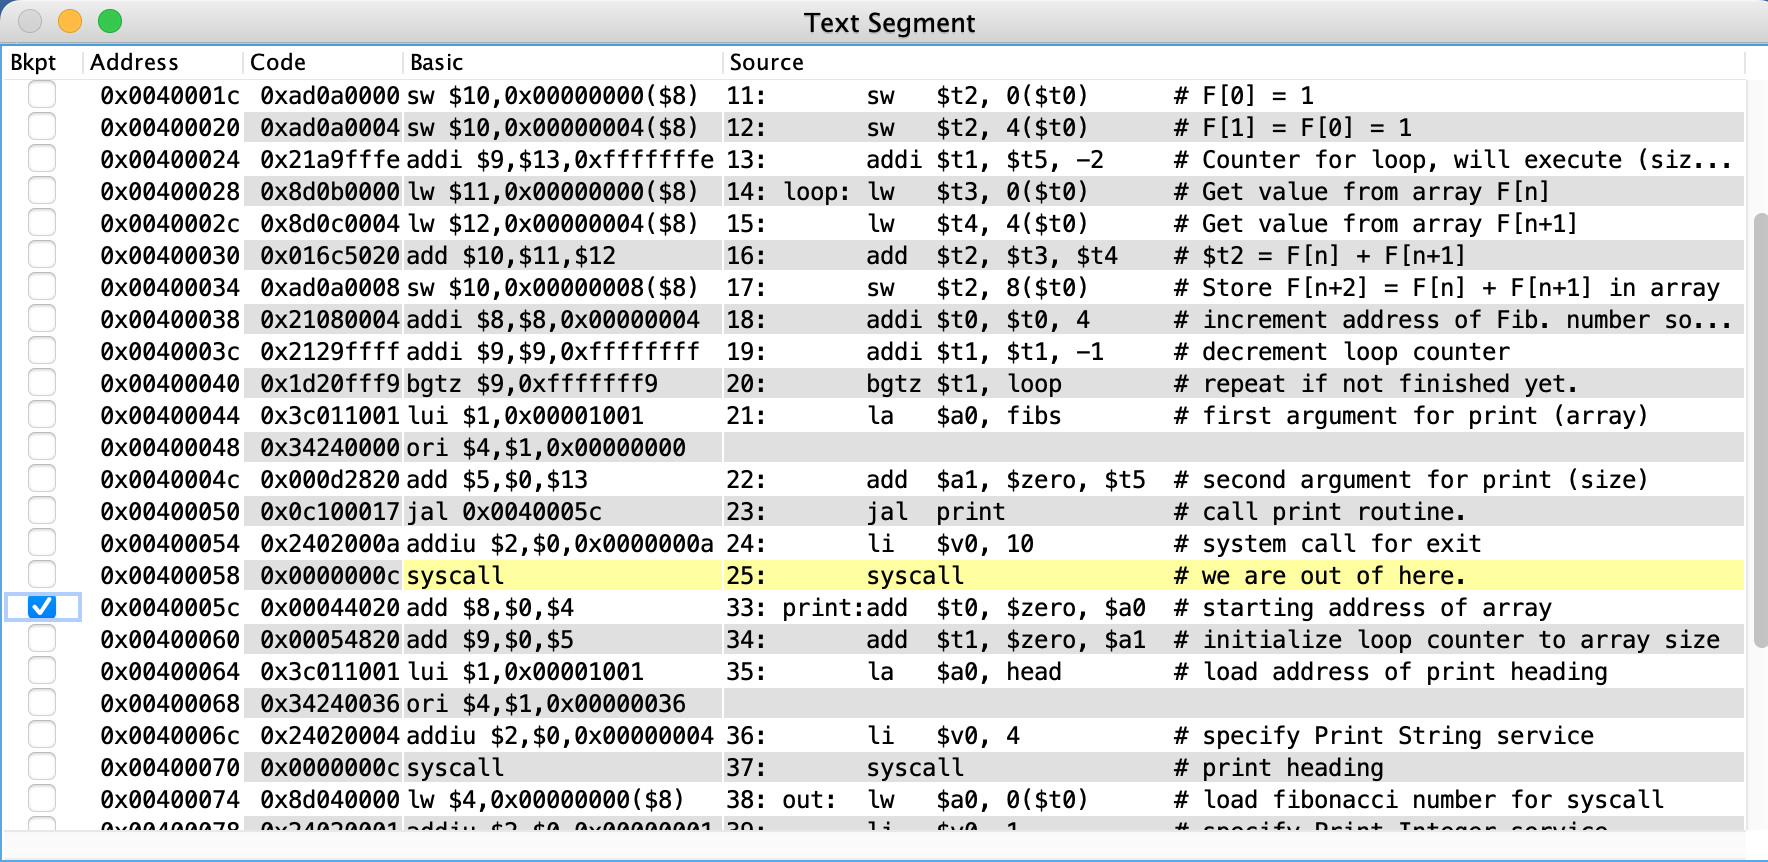
\includegraphics[width=0.8\textwidth]{27.png}

        \item[$\bullet$] Reset        
\includegraphics[width=0.04\textwidth]{20.png} and re-run 
\includegraphics[width=0.04\textwidth]{18.png} the program, which stops at the breakpoint.
    \end{itemize}
            \begin{center}
            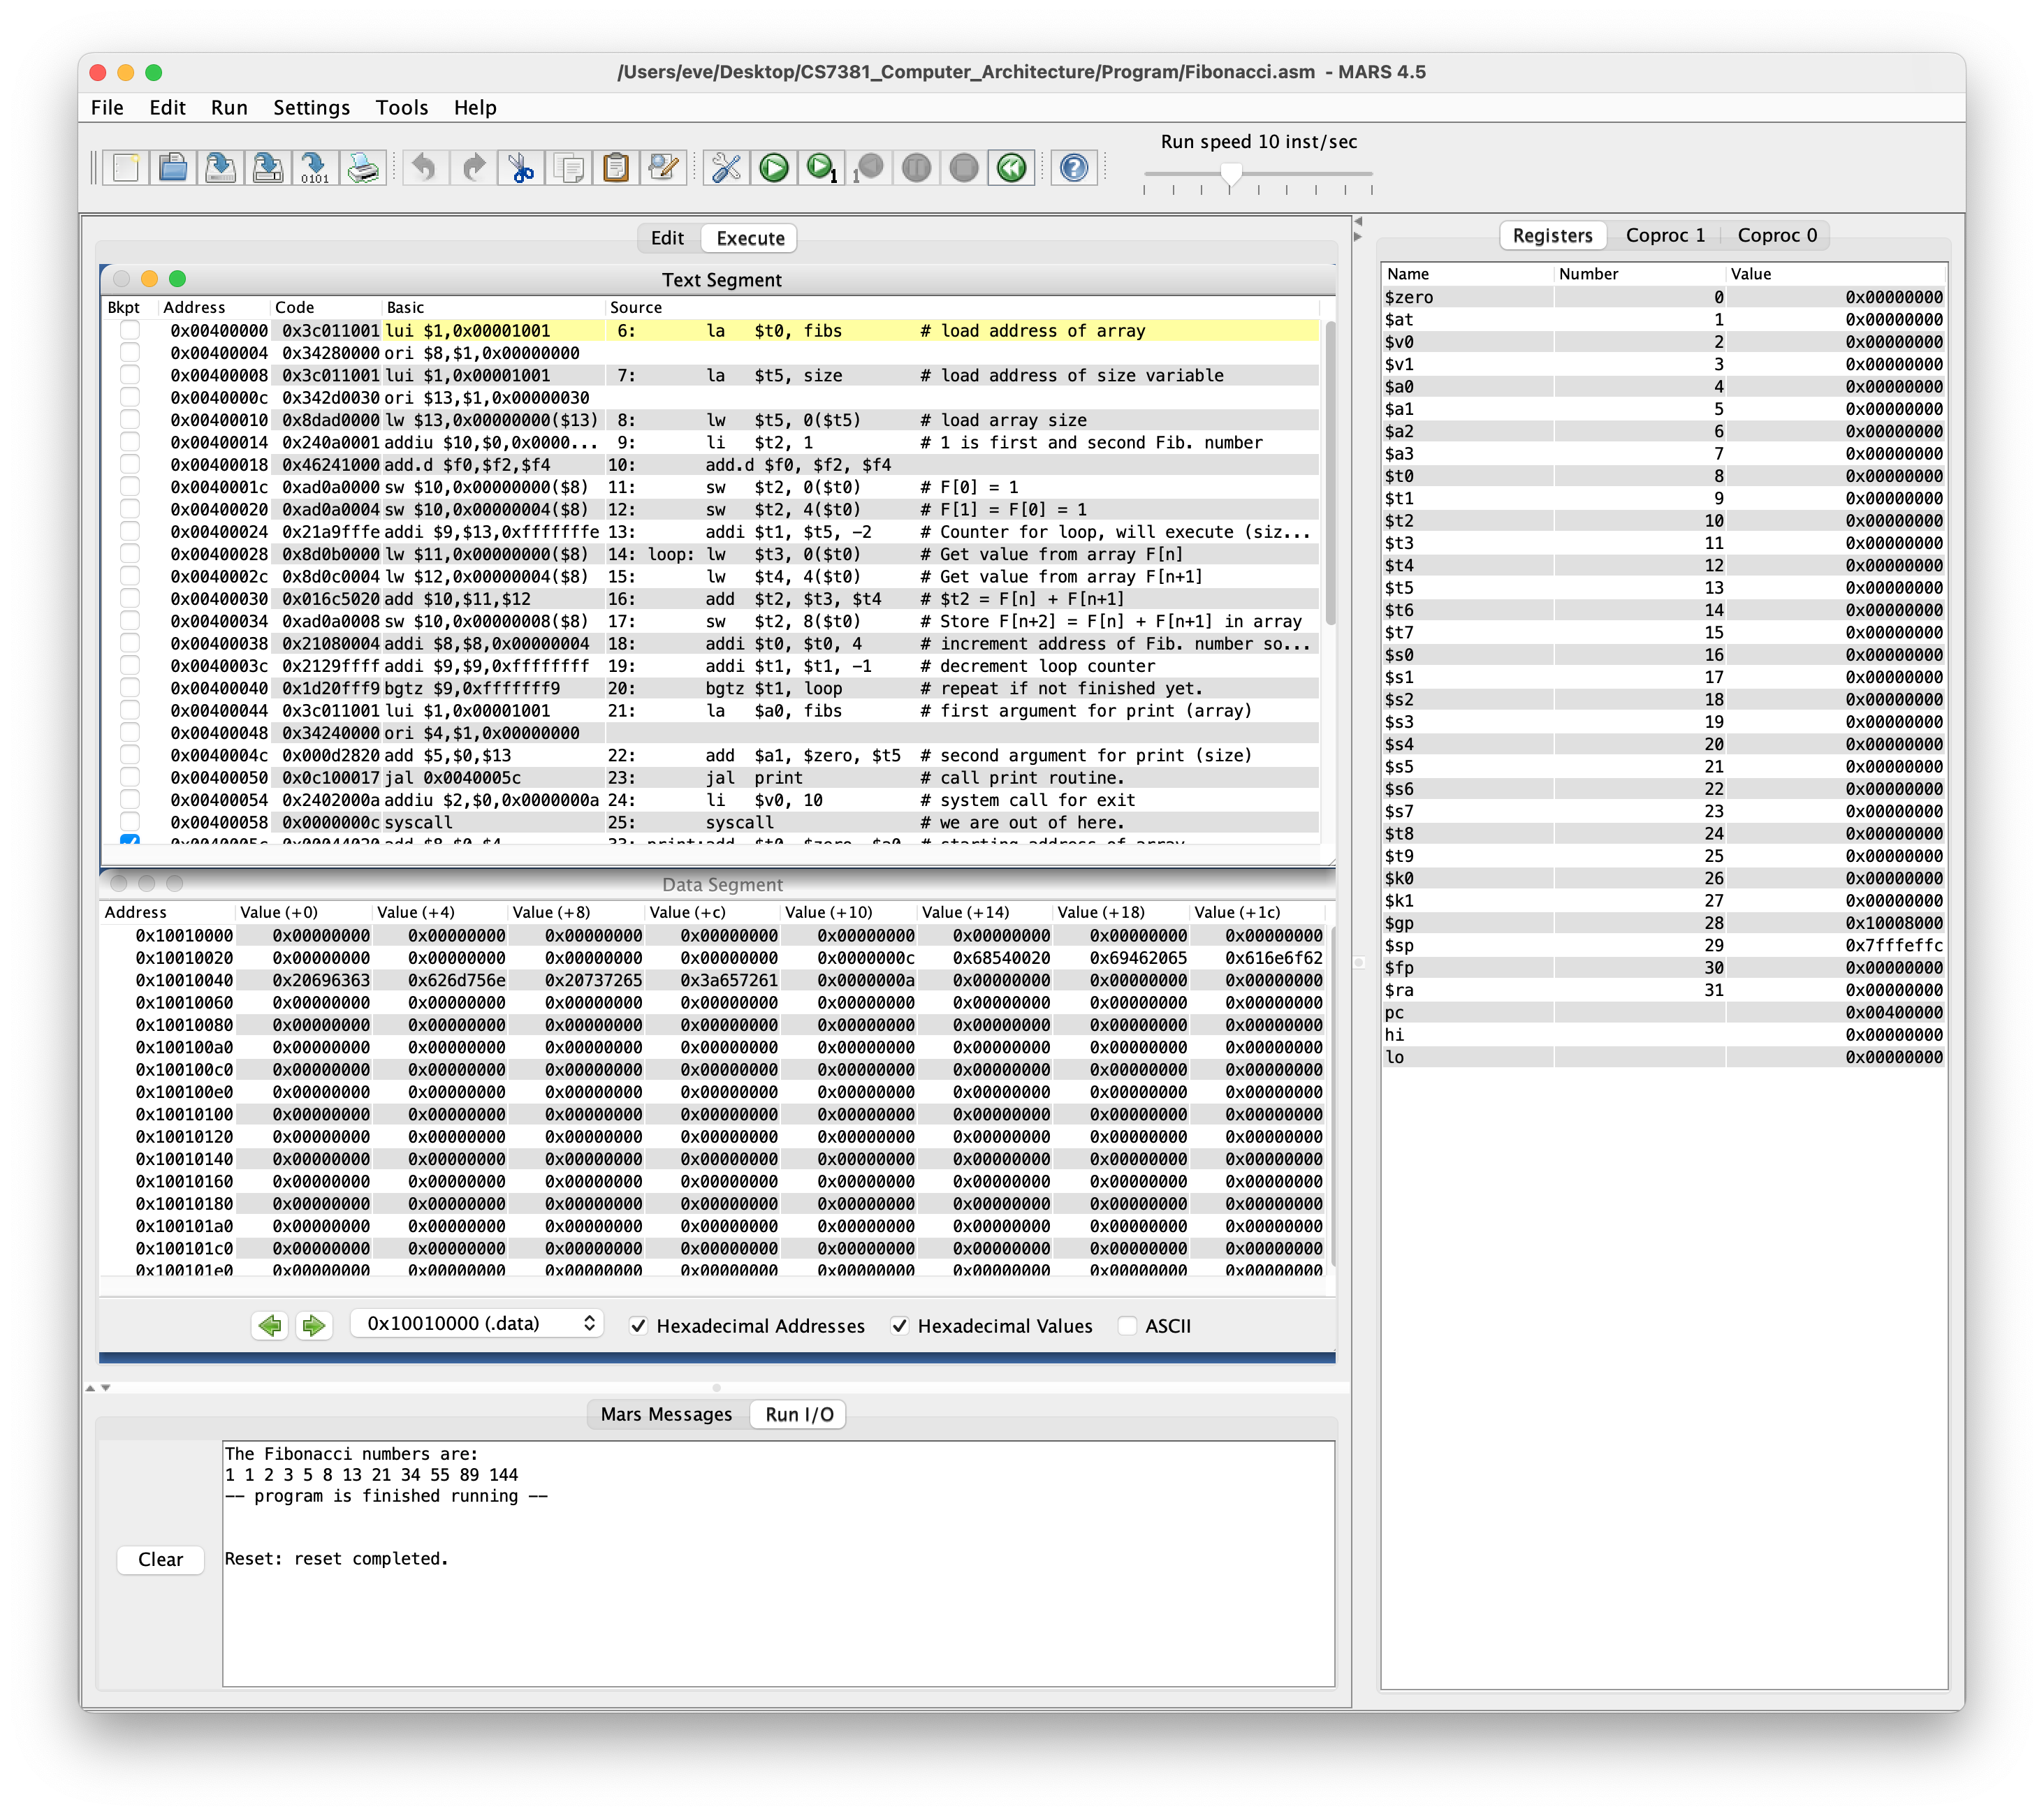
\includegraphics[width=0.9\textwidth]{28.png}
            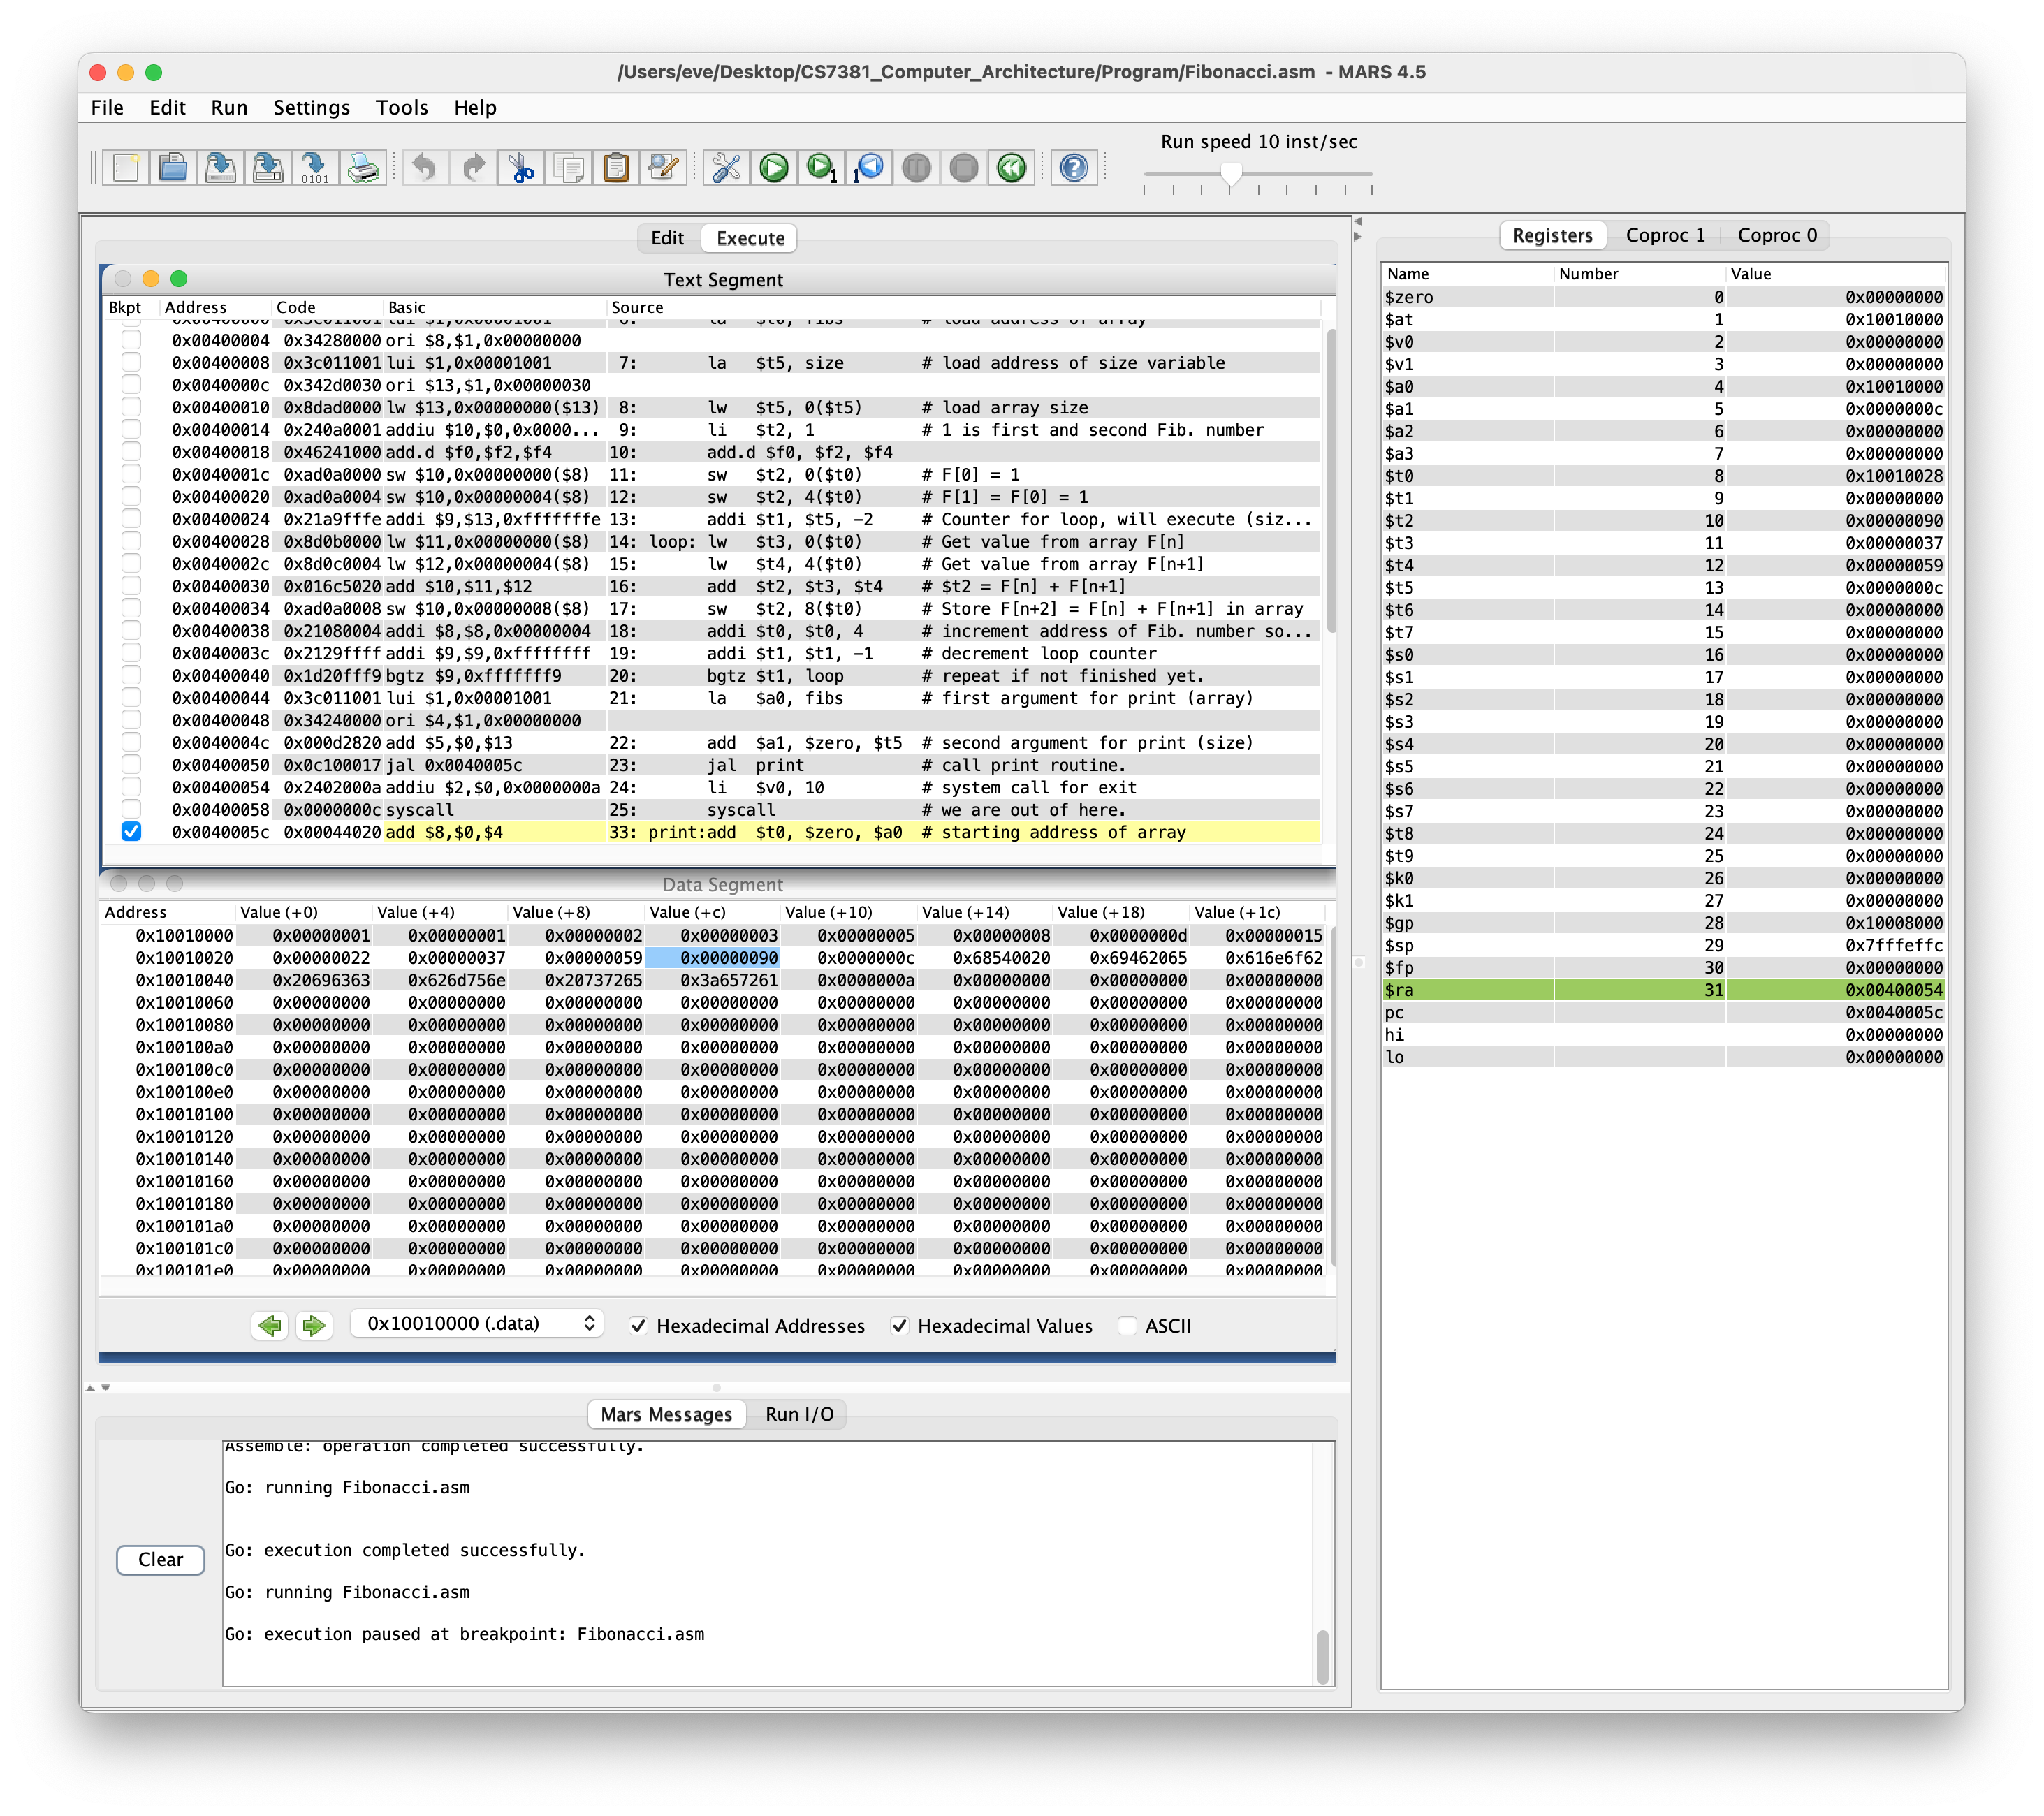
\includegraphics[width=0.9\textwidth]{29.png}
         \end{center}

    \begin{itemize}
        \item[$\bullet$] Double-click in one of the memory locations containing the computed Fibonacci numbers. The cell will be highlighted and will accept keyboard entry, similar to a spreadsheet. Enter some noticeably different value, and use the Enter key or click outside the cell to indicate that the change is complete. Example: Memory address $0x10010020 = 268501024_{ten}$ presently contains data $0x00000022 = 34_{ten}$.
    \end{itemize}
            \begin{center}
            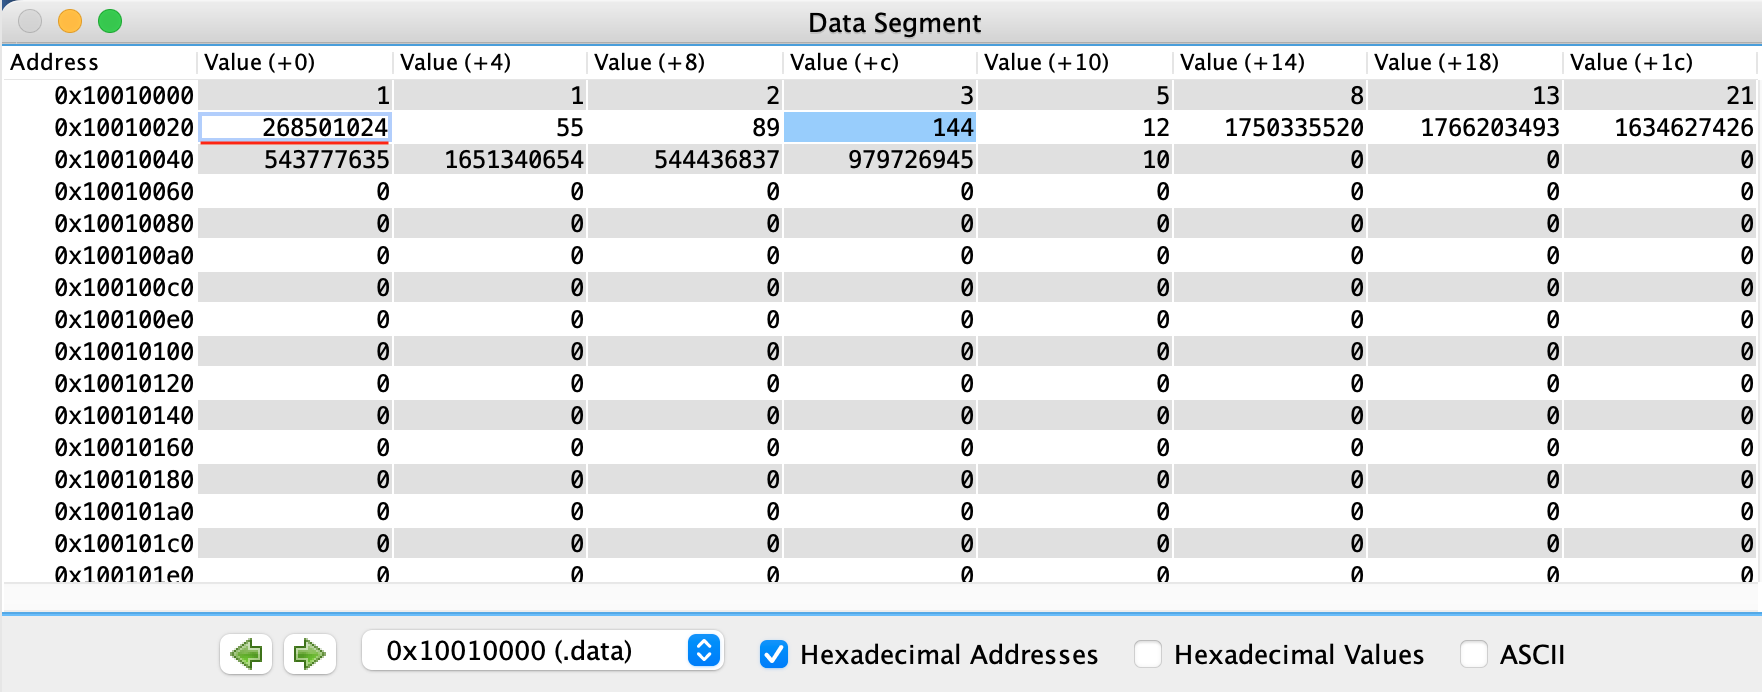
\includegraphics[width=0.8\textwidth]{30.png}
         \end{center}

    \begin{itemize} 
        \item[$\bullet$] Click 
\includegraphics[width=0.04\textwidth]{18.png} to continue from the breakpoint. The program output includes your entered value instead of the computed Fibonacci number.
    \end{itemize}
        \begin{center}
            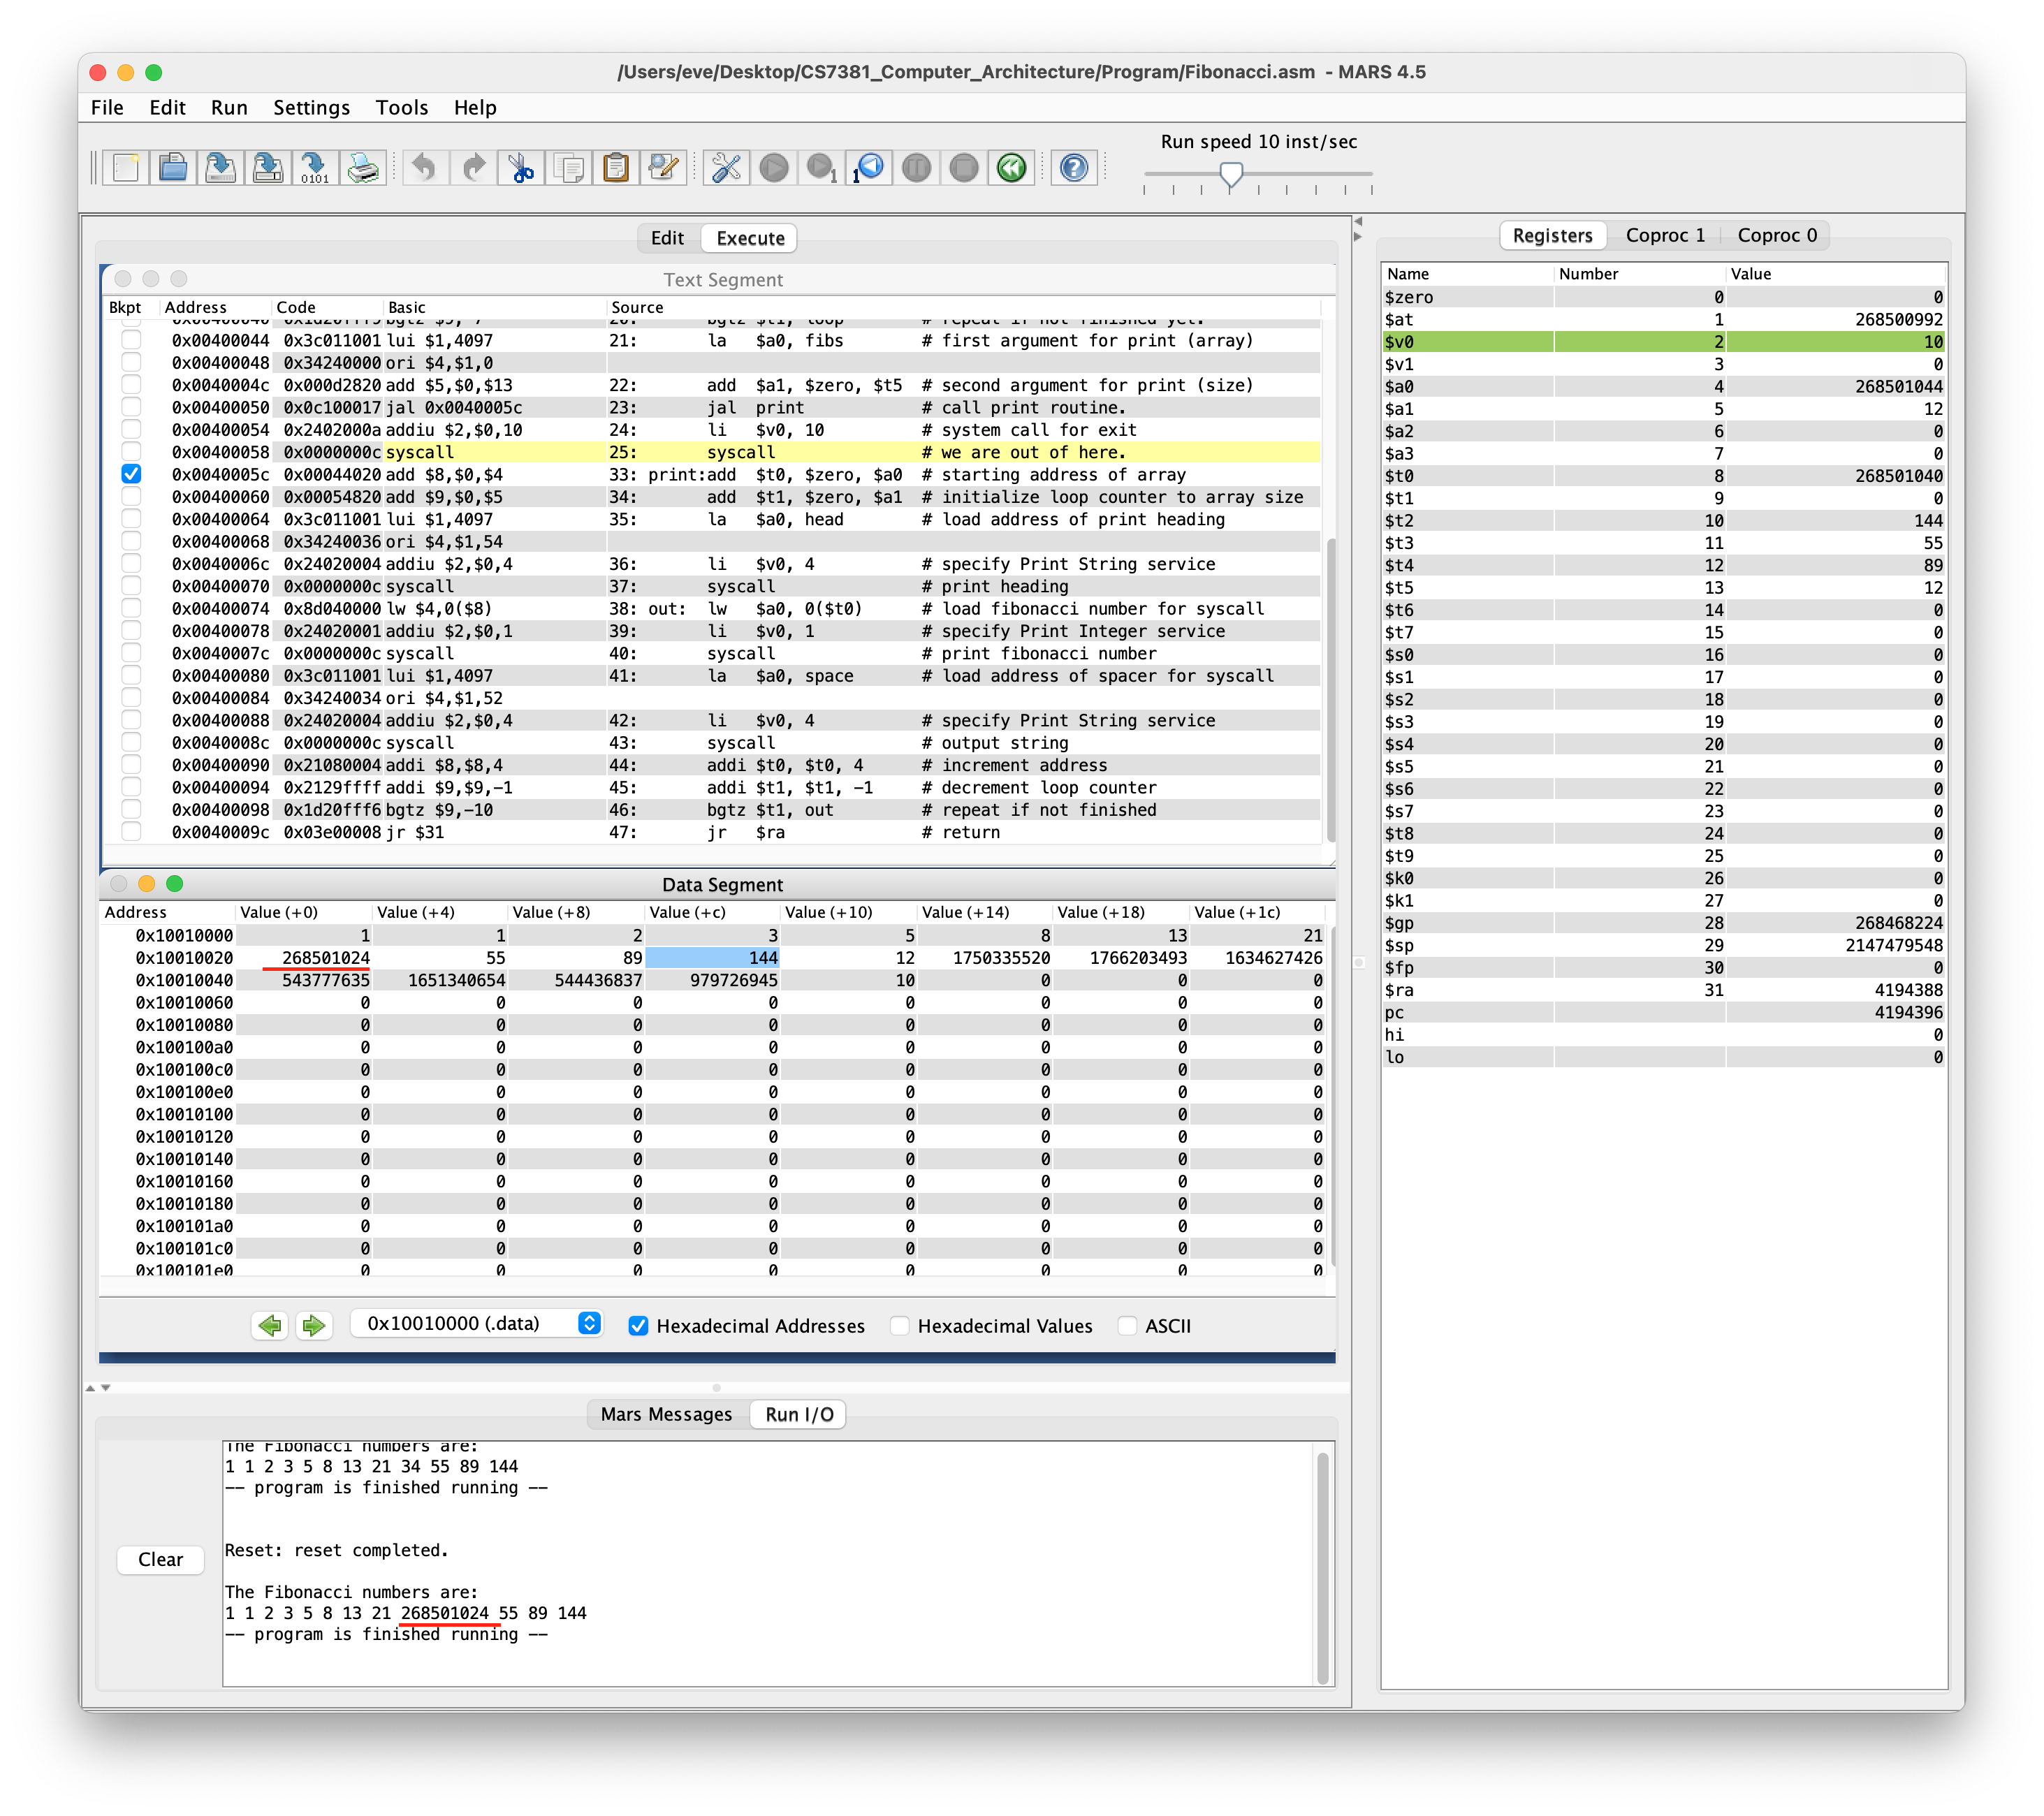
\includegraphics[width=0.9\textwidth]{31.png}
         \end{center}
    \newpage
    \item Open the Help 
\includegraphics[width=0.04\textwidth]{32.png} for information on MIPS instructions, pseudoinstructions, directives, and syscalls.
            \begin{center}
            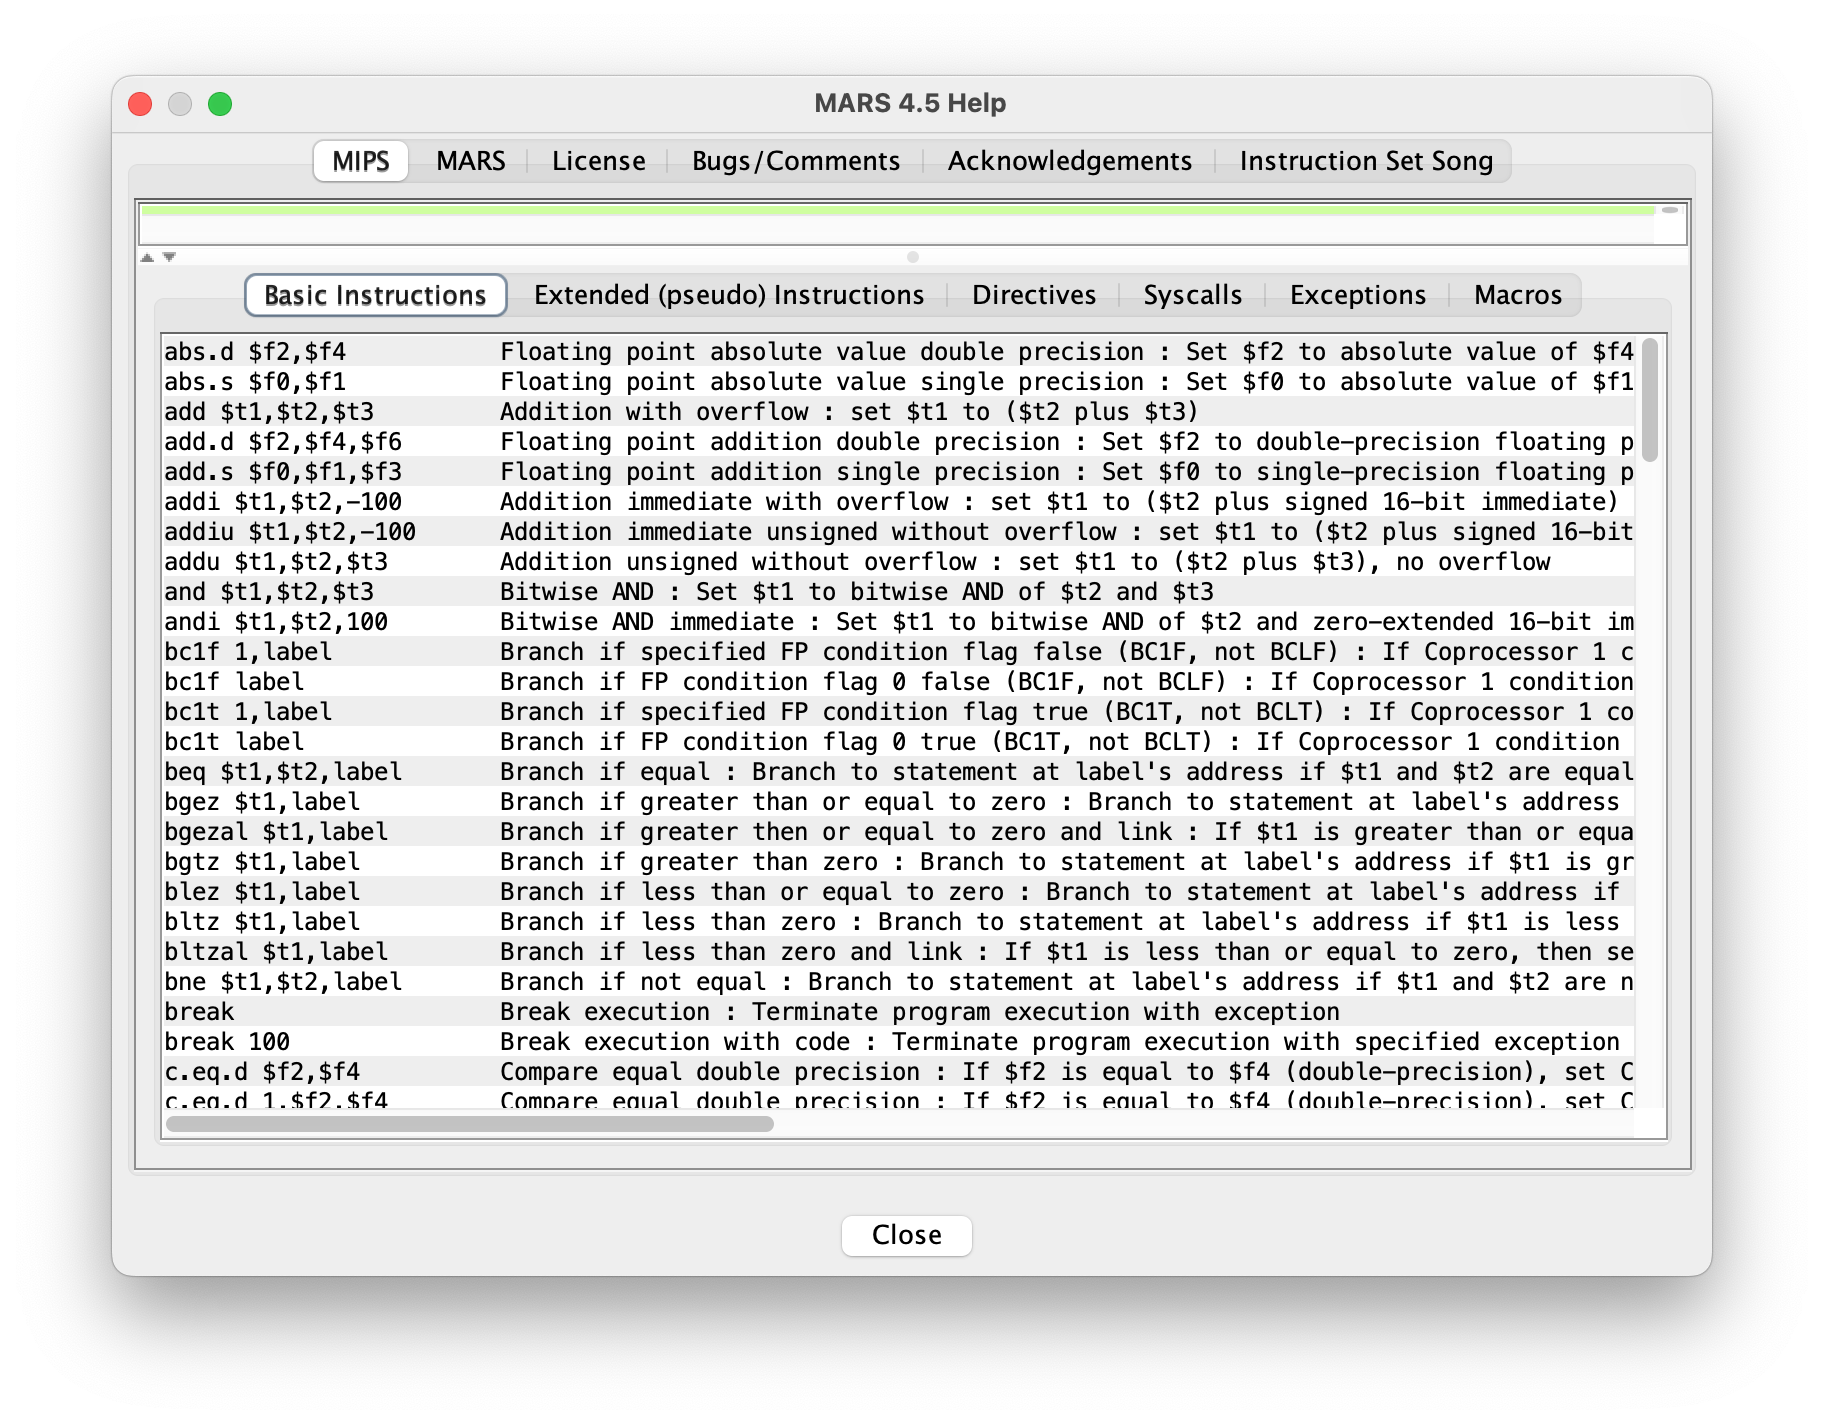
\includegraphics[width=0.9\textwidth]{33.png}
         \end{center}
    

\end{enumerate}



\end{document}
